%----------------------------------------------------------------------------------------
%	PACKAGES AND OTHER DOCUMENT CONFIGURATIONS
%----------------------------------------------------------------------------------------

\documentclass[a4paper]{article}

\usepackage[version=4]{mhchem}
\usepackage[T1]{fontenc} % Use 8-bit encoding that has 256 glyphs
\usepackage{lmodern}
\usepackage[hyphens]{url}
\usepackage{subcaption}
\usepackage{graphicx}
\linespread{1.05} % Line spacing - Palatino needs more space between lines
\usepackage{microtype} % Slightly tweak font spacing for aesthetics
\usepackage[spanish]{babel} % Language hyphenation and typographical rules
\usepackage[numbib,notlof,notlot,nottoc]{tocbibind} % Shows bibliography as a section
\usepackage[hmarginratio=1:1,top=32mm,columnsep=20pt]{geometry} % Document margins
\usepackage[section]{placeins}
\usepackage{float}
\usepackage{booktabs} % Horizontal rules in tables
\usepackage{enumitem} % Customized lists
\usepackage{fancyhdr} % Headers and footers

\pagestyle{fancy} % All pages have headers and footers
\fancyhead{} % Blank out the default header
\fancyfoot{} % Blank out the default footer
\fancyhead[C]{Ejercicios de F\'isica Te\'orica 1 $\bullet$ Ignacio Poggi} % Custom header text
\fancyfoot[C]{\thepage} % Custom footer text

\usepackage{titling} % Customizing the title section
\usepackage{hyperref} % For hyperlinks in the PDF

%----------------------------------------------------------------------------------------
%	TITLE SECTION
%----------------------------------------------------------------------------------------

\setlength{\droptitle}{-4\baselineskip} % Move the title up

\title{Ejercicios de F\'isica Te\'orica 1} % Article title
\author{%
\textsc{Ignacio Poggi} \\[1ex] % Your name
\normalsize \href{mailto:ignaciop.3@gmail.com}{ignaciop.3@gmail.com} % Your email address
}

\date{\today} % Leave empty to omit a date
\renewcommand{\maketitlehookd}{%
\begin{abstract}
\noindent Ejercicios resueltos de las gu\'ias de F\'isica Te\'orica 1 (1C/2024). Basados en algunos apuntes encontrados de las pr\'acticas de Juan Zanella (2011) y Paula Villar (2020).
\end{abstract}
}

%----------------------------------------------------------------------------------------

\begin{document}
\maketitle

% Print the title


%----------------------------------------------------------------------------------------
%	INCLUDES
%----------------------------------------------------------------------------------------
\section{Simetr\'ias. Leyes de Gauss y Amp\`ere}
\subsection{}
Los \'items a) y b) son esferas cargadas, por lo tanto tienen simetr\'ia esf\'erica. Cualquier eje que pase por el origen es un eje de simetr\'ia de rotaci\'on, as\'i como cualquier plano que contenga al origen es un plano de simetr\'ia.\newline

Esto nos permite concluir, hasta aqu\'i, que el campo el\'ectrico $\mathbf{E}$ debe apuntar y depender de la direcci\'on radial, es decir

$$ \mathbf{E}(\mathbf{r}) = E(r)\hat{r}$$

En estos sistemas, si la distribuci\'on de carga es conocida podemos calcular el campo a trav\'es de la ley de Gauss:

\begin{equation}
    \label{eq:gauss}
    \int_{S} d^{2}r' \textbf{n}' \cdot \mathbf{E(\mathbf{r})} = 4\pi Q_{V}
\end{equation}

donde $Q_{V}$ es la carga contenida en el interior de la esfera. Supongamos que la carga encerrada es $Q(r)$, el lado derecho de la ecuaci\'on (\ref{eq:gauss}) en coordenadas esf\'ericas es

$$\int_{S} d^{2}r' \textbf{n}' \cdot \mathbf{E(\mathbf{r})} = \int_{S}dS E(r) = E(r) 4\pi r^{2}$$

Luego, igualando ambos lados, obtenemos el m\'odulo del campo general para este tipo de simetr\'ias

$$E(r) 4\pi r^{2} = 4\pi Q(r) \Rightarrow E(r) = \frac{Q(r)}{r^{2}}$$

\begin{itemize}
    \item Para la esfera cargada en volumen de radio $R$, definimos la carga total como $Q \equiv Q(R)$. Si $r \geq R$, entonces la carga encerrada es $Q(r) = Q$. Si $r \leq R$:
    $$ Q(r) = \frac{4\pi}{3} r^{3} \frac{Q}{\frac{4\pi}{3} R^{3}} = Q \frac{r^{3}}{R^{3}}$$

    \begin{figure}[H]
  \centering
  \begin{subfigure}[b]{0.4\linewidth}
    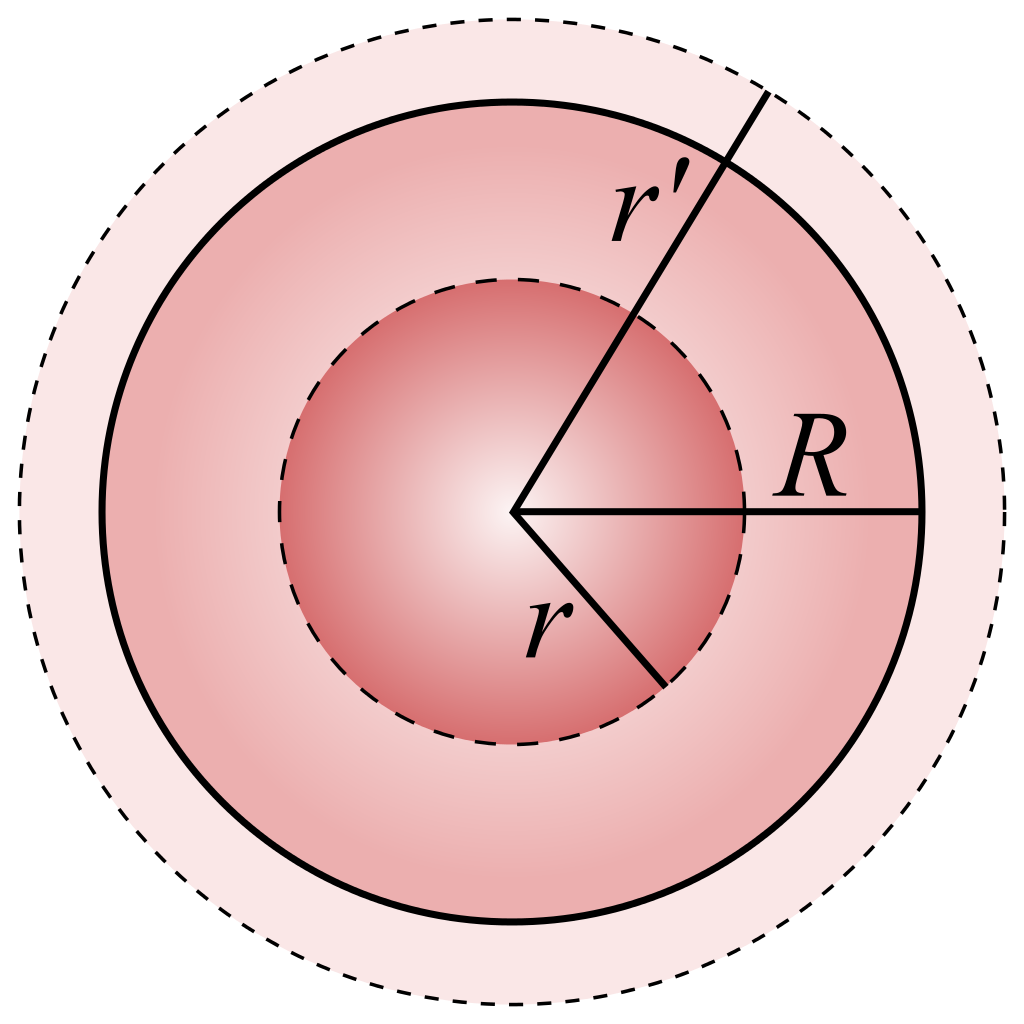
\includegraphics[width=\linewidth]{Guia1/esfera_gauss.png}
  \end{subfigure}
  \caption{Dos superficies gaussianas esf\'ericas alrededor de una esfera uniformemente cargada de radio $R$; una exterior con radio $r'$ y otra interior de radio $r$.}
  \label{fig:esfera_gauss}
\end{figure}

    Por lo tanto, la carga total y el m\'odulo del campo \textbf{E} en cada regi\'on nos queda de la siguiente manera:

    \[Q(r)=
        \begin{cases}
            Q \frac{r^{3}}{R^{3}} & r \leq R\\
            Q  & r \geq R
        \end{cases}
    \]

    \[E(r)=
        \begin{cases}
            Q \frac{r}{R^{3}} & r \leq R\\
            \frac{Q}{r^{2}} & r \geq R
        \end{cases}
    \]

 \begin{figure}[H]
  \centering
  \begin{subfigure}[b]{0.6\linewidth}
    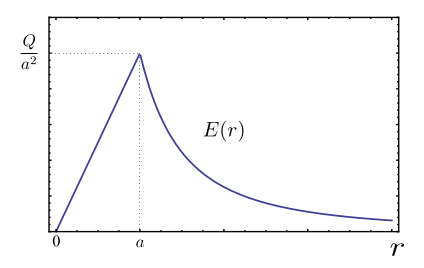
\includegraphics[width=\linewidth]{Guia1/er.png}
  \end{subfigure}
  \caption{M\'odulo del campo el\'ectrico en una esfera uniformemente cargada en volumen ($a = R$). Notemos que el campo es continuo en $r = R$.}
  \label{fig:er}
\end{figure}

Para el c\'alculo del potencial escalar, vamos a utilizar la f\'ormula general de la integral de l\'inea de \textbf{E}:

$$\Phi(r) = - \int_{\mathbf{r_{0}}}^{\mathbf{r}} d\mathbf{l}' \cdot \mathbf{E(r')}$$

En un campo radial, la componente que interesa es $r$ y el punto de referencia $\mathbf{r}_{0} \rightarrow \infty$ (ya que el campo decae como $\frac{1}{r}$ en el infinito), por lo tanto

$$\Phi(r) = \int_{r}^{\infty} dr' E(r')$$

Para nuestro caso particular, 

\[\Phi(r)=
        \begin{cases}
            \int_{r}^{\infty} dr' \frac{Q}{r'^{2}} = \frac{Q}{r} & r \geq R\\
             \int_{R}^{\infty} dr' \frac{Q}{r'^{2}} +  \int_{r}^{R} dr' \frac{r'}{R^{3}}Q = \frac{Q}{R} + \frac{Q}{2R}(1 - \frac{r^{2}}{R^{2}}) & r \leq R
        \end{cases}
    \]

\begin{figure}[H]
  \centering
  \begin{subfigure}[b]{0.6\linewidth}
    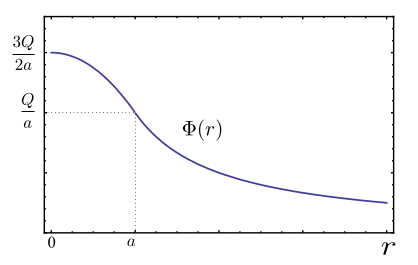
\includegraphics[width=\linewidth]{Guia1/phir.png}
  \end{subfigure}
  \caption{Potencial el\'ectrico en una esfera uniformemente cargada en volumen ($a = R$).}
  \label{fig:phir}
\end{figure}

\item En el \'item b) tenemos la esfera cargada uniformemente en superficie (densidad $\sigma$), por lo tanto la carga encerrada y el campo el\'ectrico dentro de la esfera es 0, entonces:

\[Q(r)=
        \begin{cases}
            0 & r < R\\
            Q = 4\pi R^{2}\sigma & r > R
        \end{cases}
    \]

    \[E(r)=
        \begin{cases}
            0 & r \leq R\\
            \frac{Q}{r^{2}} & r > R
        \end{cases}
    \]

Con respecto al potencial el\'ectrico del cascar\'on:

\[\Phi(r)=
        \begin{cases}
            \int_{r}^{\infty} dr' \frac{Q}{r'^{2}} = \frac{Q}{r} & r \geq R\\
             \int_{R}^{\infty} dr' \frac{Q}{r'^{2}} = \frac{Q}{R} & r \leq R
        \end{cases}
    \]

\begin{figure}[H]
  \centering
  \begin{subfigure}[b]{0.8\linewidth}
    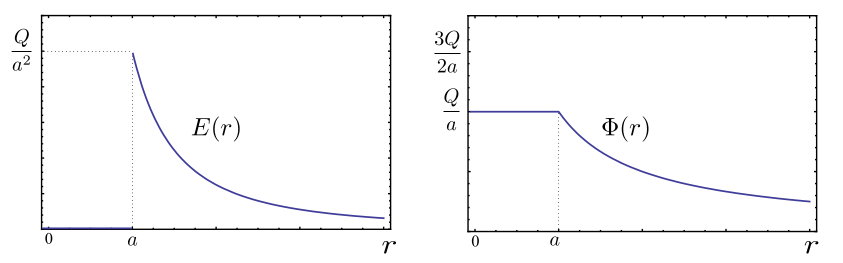
\includegraphics[width=\linewidth]{Guia1/ephir.png}
  \end{subfigure}
  \caption{Campo y potencial el\'ectrico para una esfera cargada en superficie ($a = R$) con carga $Q$.}
  \label{fig:ephir}
\end{figure}

\item En el \'item c), tenemos un plano infinito cargado uniformemente con densidad $\sigma$

\begin{figure}[H]
  \centering
  \begin{subfigure}[b]{0.5\linewidth}
    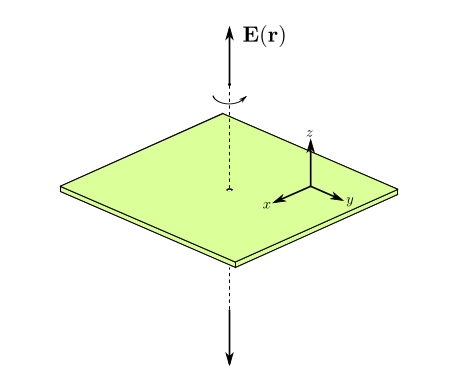
\includegraphics[width=\linewidth]{Guia1/eplano.png}
  \end{subfigure}
  \caption{Esquema del campo el\'ectrico de un plano.}
  \label{fig:eplano}
\end{figure}

Dado que el plano tiene simetr\'ia de rotaci\'on respecto a cualquier eje perpendicular, en particular el eje $z$, el campo en dicho punto debe estar sobre eje y seg\'un la normal al plano. Adem\'as, tenemos simetr\'ia de traslaci\'on sobre el plano, por lo tanto podemos decir que

$$\mathbf{E(r)} = E(z)\hat{z}$$

Para calcular el m\'odulo $E(z)$, armamos una superficie de Gauss cil\'indrica sim\'etrica respecto del plano, como indica la siguiente figura

\begin{figure}[H]
  \centering
  \begin{subfigure}[b]{0.5\linewidth}
    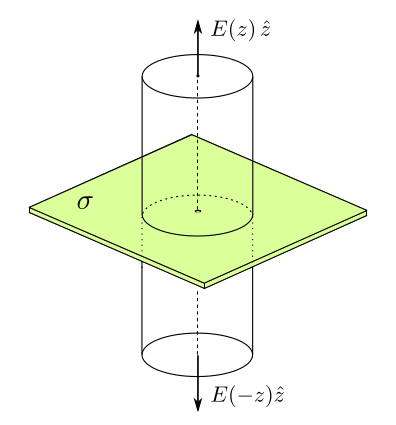
\includegraphics[width=\linewidth]{Guia1/eplano_gauss.png}
  \end{subfigure}
  \caption{Esquema de la superficie de Gauss elegida para el plano infinito con densidad uniforme $\sigma$.}
  \label{fig:eplano_gauss}
\end{figure}

Para calcular el flujo del campo el\'ectrico, tenemos tres superficies a tener en cuenta: las tapas (de \'area $A$, por ejemplo) y el lateral del cilindro. \'Esta \'ultima no contribuye a la integral porque el campo en esta regi\'on es perpendicular a la normal del plano.\newline
Las dos tapas contribuyen de la misma manera al c\'alculo (una en $z$ y la otra en $-z$), por lo cual el flujo de $\mathbf{E}$ ser\'a dos veces el flujo sobre cualquiera de las dos:

$$\int_{z' = z} d^{2}r'\mathbf{n} \cdot \mathbf{E(r')} = \mathbf{n} \cdot E(z)\hat{z} = 4\pi Q_{enc}$$

Destaquemos que, si $z > 0 \Rightarrow \mathbf{n} = \hat{z}$; y si $z < 0 \Rightarrow \mathbf{n} = -\hat{z}$, luego $\mathbf{n} = sgn(z)\hat{z}$. Entonces, la integral nos queda:

$$\int_{z' = z} d^{2}r'\mathbf{n} \cdot \mathbf{E(r')} = 2AE(z)sgn(z) = 4\pi Q_{enc}$$

Como la carga encerrada en la secci\'on circular es $Q_{enc} = \sigma A$, entonces:

$$2AE(z)sgn(z) = 4\pi \sigma A \Rightarrow E(z) = 2\pi sgn(z)$$

$$\Rightarrow \mathbf{E(r)} = 2\pi \sigma sgn(z)\hat{z}$$

Para calcular el potencial, como el campo no decae en el infinito, el punto de referencia ser\'a $z_{0} = 0$

$$\Phi(z) = -\int_{z_{0}}^{z} dz' E(z') = -2\pi \sigma \int_{0}^{z} dz' sgn(z') = -2\pi \sigma |z|$$

\begin{figure}[H]
  \centering
  \begin{subfigure}[b]{0.6\linewidth}
    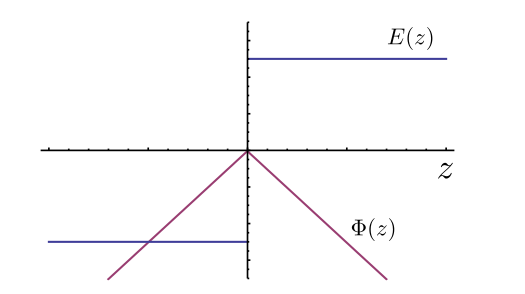
\includegraphics[width=\linewidth]{Guia1/ephi_plano.png}
  \end{subfigure}
  \caption{Campo y potencial el\'ectrico para un plano cartesiano cargado con densidad uniforme $\sigma$.}
  \label{fig:ephi_plano}
\end{figure}

Los \'items c), d) y e) tienen simetr\'ia cil\'indrica. Esto quiere decir que pueden ser
descriptas por una densidad que s\'olo depende de la distancia $\rho$ al eje de simetría $z$. Usando dos reflexiones por planos perpendiculares (como se muestra en la figura), el campo solo puede depender de la direcci\'on radial:

\begin{figure}[H]
  \centering
  \begin{subfigure}[b]{0.6\linewidth}
    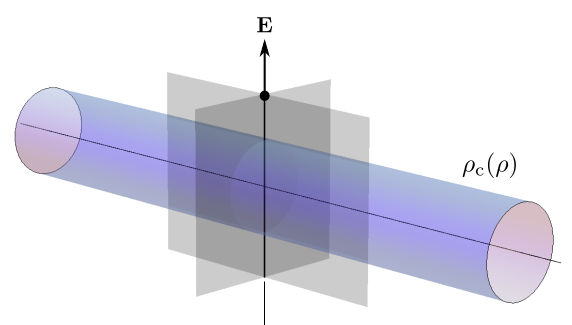
\includegraphics[width=\linewidth]{Guia1/ecilindro.png}
  \end{subfigure}
  \caption{Planos perpendiculares (uno que contiene al eje de simetr\'ia de la
distribuci\'on, y otro perpendicular) en configuraciones cil\'indricas.}
  \label{fig:ecilindro}
\end{figure}

Sobre cada uno de los planos de simetr\'ia, el campo debe ser paralelo al plano. Como en cada punto hay dos de estos planos, el campo s\'olo puede estar en la direcci\'on que es com\'un a los dos, que es $\hat{\rho}$.\newline

Si tomamos el eje $z$ como el eje de simetr\'ia, entonces el campo el\'ectrico tendr\'a la siguiente forma (habiendo eliminado las dependencias en $z$ y en $\varphi$ utilizando las simetr\'ias de traslaci\'on y rotaci\'on, respectivamente, a lo largo del eje):

$$\mathbf{E(r)} = E(\rho)\hat{\rho}$$

Finalmente, aplicamos Gauss en un cilindro de radio $\rho$ encerrando la distribuci\'on cil\'indrica generalizada:

\begin{figure}[H]
  \centering
  \begin{subfigure}[b]{0.6\linewidth}
    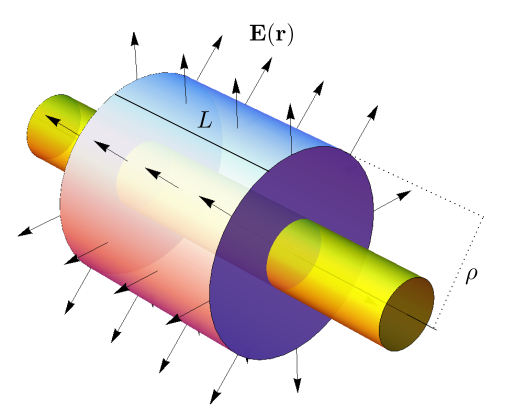
\includegraphics[width=\linewidth]{Guia1/ecilindro_gauss.png}
  \end{subfigure}
  \caption{Superficie de Gauss a lo largo del eje $z$ del cilindro para determinar $E(\rho)$.}
  \label{fig:ecilindro_gauss}
\end{figure}

Contrariamente al caso de la superficie de Gauss para el plano, aqu\'i lo que cuenta es la superficie lateral para calcular el flujo de $\mathbf{E}$ (ya que la normal en las tapas es perpendicular al mismo). El lado derecho de (\ref{eq:gauss}) nos queda:

$$2\pi \rho L E(\rho)$$

donde $L$ es la longitud del cilindro de Gauss y $\rho$ la coordenada radial. Del lado izquierdo, esto es igual a $4\pi Q_{enc}$, con $Q_{enc} = 4\pi \lambda(\rho) L$, por lo tanto:

$$ 2\pi \rho L E(\rho) = 4\pi \lambda(\rho) L \Rightarrow E(\rho) = \frac{2\lambda(\rho)}{\rho}$$

Usando este resultado, el potencial el\'ectrico se obtiene integrando a lo largo de la coordenada radial:

$$\Phi(\mathbf{r}) = \Phi(\rho) = -\int_{\rho_{0}}^{\rho}d\rho' E(\rho') = -\int_{\rho_{0}}^{\rho}d\rho' \frac{2\lambda(\rho')}{\rho'}$$

\item En d) tenemos un hilo infinito cargado con densidad lineal uniforme $\lambda(\rho') = \lambda$. En este caso, obtenemos:

$$E(\rho) = \frac{2\lambda}{\rho}$$

$$\Phi(\rho) = -\int_{\rho_{0}}^{\rho}d\rho' \frac{2\lambda}{\rho'} = -2\lambda \ln \bigg(\frac{\rho}{\rho_{0}}\bigg)$$

\begin{figure}[H]
  \centering
  \begin{subfigure}[b]{0.6\linewidth}
    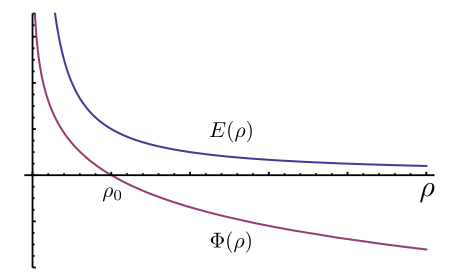
\includegraphics[width=\linewidth]{Guia1/epot_hilo1.png}
  \end{subfigure}
  \caption{$E(\rho)$ y $\Phi(\rho)$ para un hilo con densidad uniforme $\lambda$ en el eje $z$.}
  \label{fig:epot_hilo1}
\end{figure}

\item Para e) queremos calcular el campo y el potencial en el interior de un cilindro circular infinito cargado uniformemente en volumen con densidad $\rho_{c}$ (para distinguirlo de la coordenada radial $\rho$). Si definimos la carga por unidad de longitud de la siguiente manera:

$$\lambda(\rho) = \frac{1}{L} \int_{0}^{L} dz' \int_{0}^{2\pi} d\varphi' \int_{0}^{\rho} d\rho' \rho' \rho_{c}(\mathbf{r}) = 2\pi \int_{0}^{\rho} d\rho' \rho' \rho_{c}(\rho')$$

En este caso, si $a$ es el radio arbitrario del cilindro de Gauss elegido, entonces:

\[\lambda(\rho)=
        \begin{cases}
            2\pi \int_{0}^{\rho} d\rho' \rho' \rho_{c} = \pi \rho^{2} \rho_{c} = \lambda \frac{\rho^{2}}{a^{2}} & \rho \leq a\\
             \pi a^{2} \rho_{c} = \lambda & \rho \geq a
        \end{cases}
    \]

si $\lambda = 2\pi a^{2} \rho_{c}$. Con este resultado, el campo y potencial el\'ectrico nos queda:

\[\ E(\rho)=
        \begin{cases}
            2\lambda \frac{\rho}{a^{2}} & \rho \leq a\\
             \frac{2\lambda}{\rho} & \rho \geq a
        \end{cases}
    \]

\[\Phi(\rho)=
        \begin{cases}
            -\lambda \frac{\rho^{2}}{a^{2}} & \rho \leq a\\
             -\lambda - 2\lambda \ln \frac{\rho}{a} & \rho \geq a
        \end{cases}
    \]

\begin{figure}[H]
  \centering
  \begin{subfigure}[b]{0.6\linewidth}
    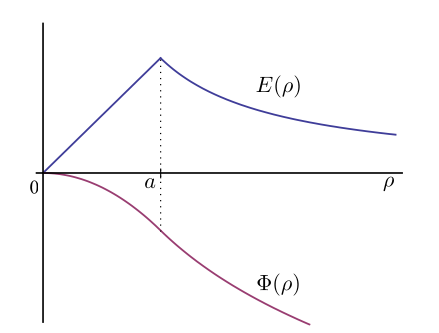
\includegraphics[width=\linewidth]{Guia1/epot_hilo2.png}
  \end{subfigure}
  \caption{$E(\rho)$ y $\Phi(\rho)$ para un hilo con densidad uniforme en volumen $\lambda$ en el eje $z$.}
  \label{fig:epot_hilo2}
\end{figure}

\item En f) nos dan un cilindro circular infinito de radio $a$, cargado uniformemente en superficie (densidad $\sigma$). La carga encerrada por unidad de longitud nos queda:

\[\lambda(\rho)=
        \begin{cases}
            0 & \rho \leq a\\
             2\pi \sigma & \rho \geq a
        \end{cases}
    \]

entonces, 

\[\ E(\rho)=
        \begin{cases}
            0 & \rho \leq a\\
             \frac{2\lambda}{\rho} & \rho \geq a
        \end{cases}
    \]

\[\Phi(\rho)=
        \begin{cases}
            0 & \rho \leq a\\
             - 2\lambda \ln \frac{\rho}{a} & \rho \geq a
        \end{cases}
    \]

\begin{figure}[H]
  \centering
  \begin{subfigure}[b]{0.6\linewidth}
    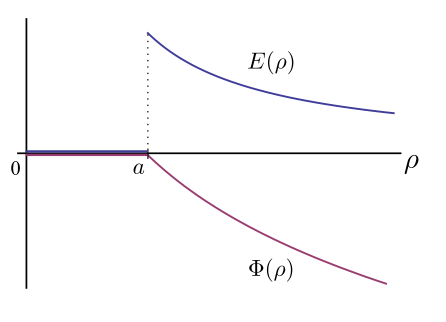
\includegraphics[width=\linewidth]{Guia1/epot_hilo3.png}
  \end{subfigure}
  \caption{$E(\rho)$ y $\Phi(\rho)$ para un hilo con densidad uniforme en superficie $\sigma$ en el eje $z$.}
  \label{fig:epot_hilo3}
\end{figure}

\end{itemize}

\subsection{}

Como hicimos en el ejercicio anterior, y siguiendo los apuntes de Zanella; agrupemos los \'items a), d) y e) de simetr\'ia cil\'indrica (de traslaci\'on y rotaci\'on con respecto a un eje, como puede ser por ejemplo, $z$) y antisim\'etricos respecto de los planos perpendiculares a ese eje.

\begin{figure}[H]
  \centering
  \begin{subfigure}[b]{0.8\linewidth}
    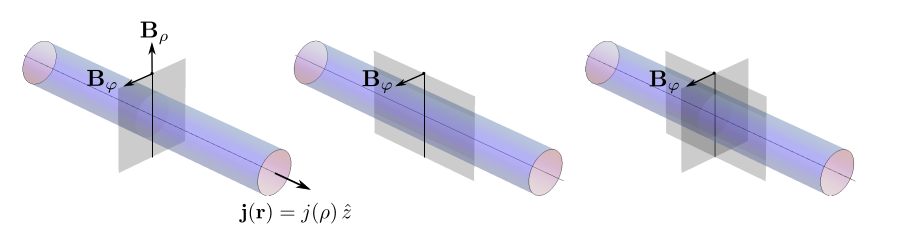
\includegraphics[width=\linewidth]{Guia1/b_sim.png}
  \end{subfigure}
  \caption{Planos perpendiculares respecto del eje de simetr\'ia de una configuraci\'on cil\'indrica.}
  \label{fig:b_sim}
\end{figure}

En el plano perpendicular al eje de la distribuci\'on, la corriente es antisim\'etrica (si reflejamos la corriente por ese plano y cambiamos de signo, obtenemos el sistema original), lo que implica que

$$\mathbf{B(r)} = B_{\rho}\hat{\rho} + B_{\varphi}\hat{\varphi}$$

Por otro lado, en el plano que contiene al eje longitudinal, el sistema tiene simetr\'ia de reflexi\'on, por lo tanto aqu\'i $\mathbf{B}$ debe ser perpendicular, luego

$$\mathbf{B} = B_{\varphi}\hat{\varphi} = B(\rho) \hat{\varphi}$$

Como hicimos con el campo el\'ectrico, para hallar el m\'odulo del campo magn\'etico utilizaremos la ley de Amp\`ere (an\'aloga a la ley de Gauss para $\mathbf{E}$),

\begin{equation}
    \label{eq:ampere}
    \oint d\mathbf{l} \cdot \mathbf{B} = \frac{4\pi I(\rho)}{c}
\end{equation}

donde $I$ es la corriente encerrada por la espira de Amp\`ere y $c$ es la velocidad de la luz.\newline

Como tenemos simetr\'ias cil\'indricas, la espira circular ser\'a de radio $\rho$ y alrededor del eje $z$. Luego, el lado izquierdo de \ref{eq:ampere} queda (integrando en $\varphi)$

$$\oint d\mathbf{l} \cdot \mathbf{B} = 2\pi B(\rho)$$

Por otro lado, la corriente total que pasa por la circunferencia de radio $\rho$ estar\'a dada por

$$I(\rho) = 2\pi \int_{0}^{\rho} d\rho' \rho' j(\rho')$$

con $j(\rho')$ la densidad de corriente. Luego, a ambos lados de la ecuaci\'on tendremos

$$2\pi B(\rho) = \frac{4\pi I(\rho)}{c}$$
$$ \Rightarrow B(\rho) = \frac{2 I(\rho)}{c\rho}$$

Para obteener el potencial vector $\mathbf{A}$ utilizamos la ecuaci\'on del rotor:

$$\mathbf{B} = \nabla \times \mathbf{A}$$

Teniendo en cuenta la definici\'on del rotor en coordenadas cil\'indricas

$$\nabla \times \mathbf{A} = \hat{\rho}\bigg(\frac{1}{\rho}\frac{\partial A_{z}}{\partial \varphi} - \frac{\partial A_{\varphi}}{\partial z}\bigg) + \hat{\varphi}\bigg(\frac{\partial A_{\rho}}{\partial z} - \frac{\partial A_{z}}{\partial \rho}\bigg) + \hat{z}\bigg(\frac{1}{\rho}\frac{\partial (\rho A_{\varphi})}{\partial \rho} - \frac{1}{\rho}\frac{\partial A_{\rho}}{\partial \varphi}\bigg)$$

Respetando la simetr\'ia de las fuentes, y sabiendo que $\mathbf{B} = B(\rho) \hat{\varphi}$, el rotor se reduce a la coordenada $\varphi$, por lo tanto

$$B(\rho) \hat{\varphi} = \hat{\varphi}\bigg(\frac{\partial A_{\rho}}{\partial z} - \frac{\partial A_{z}}{\partial \rho}\bigg) \Rightarrow B(\rho) = - \frac{\partial A_{z}}{\partial \rho}$$

$$ \Rightarrow \mathbf{A} = A_{z}(\rho)\hat{z}$$

Integramos la ultima igualdad y obtenemos:

$$A_{z}(\rho) = - \int_{\rho_{0}}^{\rho} d\rho' B(\rho')$$

\begin{itemize}
    \item En a) tenemos un hilo infinito con corriente $I(\rho) = I$. Luego, los campos nos quedan de la siguiente manera:

    $$\mathbf{B} = \frac{2I}{c\rho}\hat{\varphi}$$

    $$\mathbf{A} = -\hat{z}\int_{\rho_{0}}^{\rho} d\rho' B(\rho') = -\hat{z} \frac{2I}{c} \int_{\rho_{0}}^{\rho} d\rho' \frac{1}{\rho'} = -\frac{2I}{c} \ln \bigg(\frac{\rho}{\rho_{0}}\bigg)\hat{z}$$

    \item En d) tenemos un cilindro circular infinito con corriente uniforme en su interior, paralela a su eje. En este caso, tenemos que calcular por separado la regi\'on interior y exterior al cilindro.

    \begin{figure}[H]
  \centering
  \begin{subfigure}[b]{0.8\linewidth}
    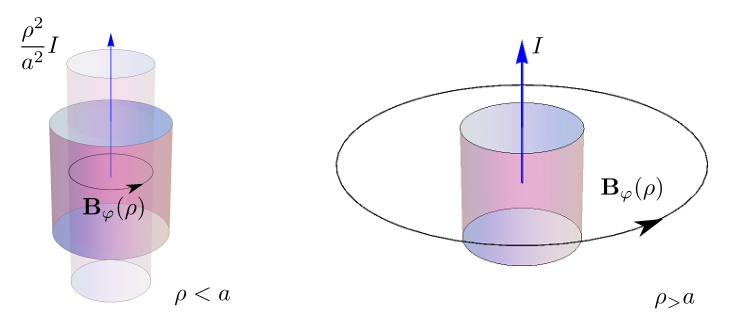
\includegraphics[width=\linewidth]{Guia1/ampere_cilindro1.png}
  \end{subfigure}
  \caption{Cilindros de Amp\`ere en la regi\'on interior y exterior a la configuraci\'on cil\'indrica con corriente uniforme.}
  \label{fig:ampere_cilindro}
\end{figure}

    La corriente que atraviesa el cilindro de radio $\rho < a$ es $I(\rho) = I \frac{\rho^{2}}{a^{2}}$. Para $\rho > a$, la corriente encerrada es la total, entonces $I(\rho) = I$ y:

    \[
        \begin{cases}
            2\pi \rho B(\rho) = \frac{4\pi}{c}I \frac{\rho^{2}}{a^{2}} & \rho \leq a\\
             2\pi \rho B(\rho) = \frac{4\pi}{c}I & \rho \geq a
        \end{cases}
    \]

    Luego, el m\'odulo del campo magn\'etico resulta

    \[B(\rho)=
        \begin{cases}
            \frac{2I}{c} \frac{\rho}{a^{2}} & \rho \leq a\\
             \frac{2I}{c\rho} & \rho \geq a
        \end{cases}
    \]

    Como tenemos un cilindro macizo, el potencial vector se calcula en dos regiones de la siguiente manera (parecido a como hicimos antes para el potencial el\'ectrico) con $\rho_{0} = 0$:

     \[A_{z}(\rho)=
        \begin{cases}
            -\int_{0}^{\rho} d\rho' B(\rho') =  -\int_{0}^{\rho} d\rho' \frac{2I\rho'}{ca^{2}} = - \frac{I\rho^{2}}{ca^{2}}  & \rho \leq a\\
              -\int_{0}^{a} d\rho' B(\rho') -\int_{a}^{\rho} d\rho' B(\rho') =  -\int_{0}^{a} d\rho' \frac{2I\rho'}{ca^{2}} -\int_{a}^{\rho} d\rho' \frac{2I}{c\rho'} = -\frac{I}{c} - \frac{2I}{c} \ln \frac{\rho}{a} & \rho \geq a
        \end{cases}
    \]

    \item En el \'item e) hay un cilindro circular infinito con corriente superficial uniforme paralela a su eje. Dentro no tenemos campo, y por fuera la corriente encerrada es la total $I$, por lo tanto los campos $\mathbf{B}$ y $\mathbf{A}$ por fuera son id\'enticos al \'item a):

    \[B(\rho)=
        \begin{cases}
            0 & \rho < a\\
             \frac{2I}{c\rho} & \rho > a
        \end{cases}
    \]

    \[A_{z}(\rho)=
        \begin{cases}
            0  & \rho \leq a\\
            -\frac{2I}{c} \ln (\frac{\rho}{a}   & \rho \geq a
        \end{cases}
    \]

    \item En b) nos dan un plano infinito con densidad de corriente superficial uniforme $\kappa$. El plano de corriente es sim\'etrico respecto de las reflexiones por planos que contengan a $\kappa$ y la normal al plano con corriente, como ejemplifica la figura:

      \begin{figure}[H]
  \centering
  \begin{subfigure}[b]{0.6\linewidth}
    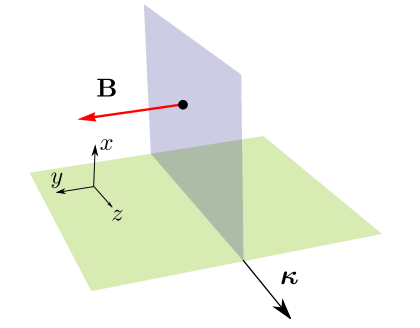
\includegraphics[width=\linewidth]{Guia1/b_plano.png}
  \end{subfigure}
  \caption{Plano infinito con densidad de corriente en superficie $\mathbf{\kappa}$ en direcci\'on $z$.}
  \label{fig:b_plano}
\end{figure}

    En un plano de simetr\'ia, $\mathbf{B}$ debe ser perpendicular, por lo tanto es de la forma

    $$\mathbf{B(r)} = B(x)\hat{y}$$

    Vemos que solo puede depender de la coordenada $x$, debido a la simetr\'ia de traslaci\'on en $y$ y $z$. Aplicando la simetr\'ia de reflexi\'on en el plano $yz$, podemos ver que 
    $$B(-x) = -B(x)$$ Aplicamos Amp\`ere a un lazo rectangular sim\'etrico respecto del plano y perpendicular a la corriente para calcular este m\'odulo:

    
      \begin{figure}[H]
  \centering
  \begin{subfigure}[b]{0.6\linewidth}
    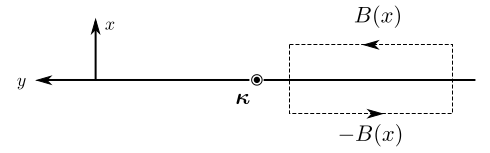
\includegraphics[width=\linewidth]{Guia1/b_plano_ampere.png}
  \end{subfigure}
  \caption{Lazo de Amp\`ere para el plano de corriente $\mathbf{\kappa}$ en $z$}
  \label{fig:b_plano_ampere}
\end{figure}

    $$\Rightarrow \oint  d\mathbf{l'} \cdot \mathbf{B} = \frac{4\pi I}{c}$$

    $$\Rightarrow 2AB(x) sgn(z) = \frac{4\pi \kappa A}{c}$$

    $$\Rightarrow B(x) = \frac{2\pi \kappa}{c} sgn(z)$$

    Para el potencial vector $\mathbf{A}$, imponemos que \'este tenga las mismas simetr\'ias que la distribuci\'on de corriente, por lo tanto $\mathbf{A} = A_{z}(x)\hat{z}$. Por otro lado,

    $$\mathbf{B} = \nabla \times \mathbf{A} = -\frac{\partial A_{z}}{\partial x}\hat{y}$$

    $$\Rightarrow -\frac{\partial A_{z}}{\partial x} = \frac{2\pi \kappa}{c} sgn(z)$$

    Integramos esta \'ultima ecuaci\'on tomando como punto de referencia $x = 0$ (cuenta id\'entica al potencial del campo el\'ectrico del plano cargado), entonces:

    $$A_{z}(x) = -\frac{2\pi \kappa}{c} |z|$$

    \item Para el \'item c), hay una corriente uniforme radial que fluye entre dos esferas conc\'entricas de radios $a$ y $b$.\newline

    Como la corriente es radial y uniforme, la densidad de corriente no depende de la direcci\'on  y es siempre la misma, es decir $\mathbf{j(r)} = j(\mathbf{r})\hat{r} = j(r)\hat{r}$ y adem\'as $4\pi r^{2} j(r) = I$.\newline

    Por simetr\'ia de rotaci\'on alrededor de cualquier eje que pase por el origen, $\mathbf{B}$ debe ser radial. Por otro lado, como ya vimos en las simetr\'ias esf\'ericas, cualquier plano que contenga al origen es un plano de simetr\'ia, luego $\mathbf{B}$ debe estar en la direcci\'on de la normal. Estas dos condiciones s\'olo pueden ser satisfechas por un campo $\mathbf{B} = 0$.

    \item En f) tenemos un solenoide infinito (circular o no) con $n$ vueltas por unidad de longitud y corriente $I$. Si consideramos cada espira plana y paralelas entre s\'i, podemos asumir que tenemos una densidad superficial de corriente $\mathbf{\kappa}$ de m\'odulo $nI$ y direcci\'on tangente al eje del solenoide.\newline

    Suponiendo el solenoide infinito longitudinal al eje $z$, la reflexi\'on por cualquier plano paralelo a $xy$ es una simetr\'ia. Como cualquier punto puede pasar por estos planos y $\mathbf{B}$ tiene que ser antisim\'etrico a ellos, solo puede tener componente en $z$.

    La simetr\'ia de traslaci\'on permite decir que $\mathbf{B}$ no puede depender de $z$, luego

    $$\mathbf{B(r)} = B(\rho, \varphi)\hat{z}$$

    De F\'isica 3 sabemos que el campo toma un valor constante $B_{int}$ dentro del solenoide y otro valor constante $B_{ext}$ en su exterior. A este resultado se llega luego de aplicar Amp\`ere a los tres lazos de la siguiente figura:

    \begin{figure}[H]
  \centering
  \begin{subfigure}[b]{0.8\linewidth}
    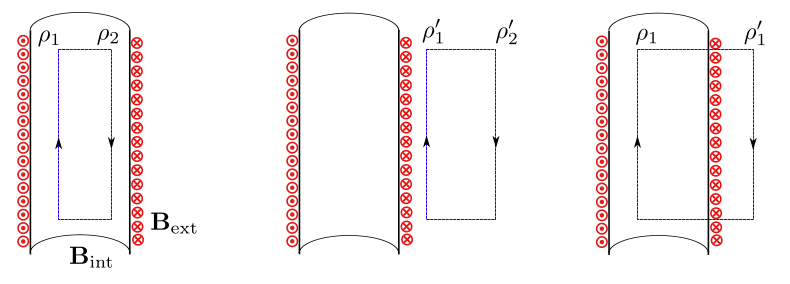
\includegraphics[width=\linewidth]{Guia1/b_solenoide.png}
  \end{subfigure}
  \caption{Lazos de Amp\`ere para las tres regiones de un solenoide infinito.}
  \label{fig:b_solenoide}
\end{figure}

    En cada uno de ellos, tenemos

    $$B_{int}(\rho_{1}) - B_{int}(\rho_{2}) = 0$$

    $$B_{ext}(\rho_{1}') - B_{ext}(\rho_{2}') = 0$$

    $$B_{int}(\rho_{1}) - B_{ext}(\rho_{1}') = \frac{4\pi nI}{c}$$

    Como el campo exterior siempre es 0, la \'ultima ecuaci\'on nos da el valor del m\'odulo de $\mathbf{B}$ que busc\'abamos:

    $$B_{int}(\rho_{1})= \frac{4\pi nI}{c}$$

    Para hallar el potencial vector $\mathbf{A}$, supongamos que el solenoide es de secci\'on circular. Dada la simetr\'ia de rotaci\'on y traslaci\'on, tenemos que

    $$\mathbf{A(r)} = A_{\rho}(\rho)\hat{\rho} + A_{\varphi}(\rho)\hat{\varphi}$$

    Debido a que el solenoide es circular, nos aseguramos que la distribuci\'on de corriente es antisim\'etrica respecto de cualquier plano que contenga al eje $z$, por lo tanto $A_{z} = A_{\rho} = 0$. Entonces,

    $$\mathbf{A(r)} = A(\rho)\hat{\varphi}$$

    $$\Rightarrow \mathbf{B} = \nabla \times \mathbf{A} = \frac{1}{\rho}\frac{\partial}{\partial \rho}(\rho A(\rho))\hat{z}$$

    $$\Rightarrow B(\rho) = \frac{4\pi nI}{c} = \frac{1}{\rho}\frac{\partial}{\partial \rho}(\rho A(\rho))$$ si $\rho < a$

    Integrando:

    \[A(\rho)= \frac{1}{\rho} \int_{0}^{\rho} d\rho' \rho' B(\rho') = \frac{4\pi nI}{c}
        \begin{cases}
            \frac{\rho}{2}  & \rho < a\\
            \frac{a^{2}}{2\rho}  & \rho \geq a
        \end{cases}
    \]

    \item En g) nos dan un toro de secci\'on circular con un total de $N$ vueltas. Cualquier plano que contenga al eje del toro (por ejemplo, el eje $z$) es un plano de simetr\'ia. Como vimos en el ejericicio anterior, ac\'a tambi\'en tendremos que $B_{ext} = 0$, y haciendo unas cuentas parecidas al solenoide, nos queda que el campo en el interior del toro ser\'a:

    $$\mathbf{B_{int}(r)} = \frac{2NI}{c\rho}\hat{\varphi}$$

    donde $I$ es la corriente total que circula por cada una de las $N$ espiras. El c\'alculo de $\mathbf{A}$ es un quilombo, as\'i que te lo debo.

\end{itemize}

\subsection{}

Para encarar este ejercicio, tengamos en cuenta las f\'ormulas generales para el potencial el\'ectrico $\Phi$ seg\'un las integrales de Poisson (lineal, superficial o volum\'etrica seg\'un corresponda):

\begin{equation}
    \label{eq:poisson_lineal}
    \Phi(\mathbf{r}) = \int_{C} dl \frac{\lambda(\mathbf{r'})}{|\mathbf{r} - \mathbf{r'}|}
\end{equation}

\begin{equation}
    \label{eq:poisson_sup}
    \Phi(\mathbf{r}) = \int_{S} d^{2}r' \frac{\sigma(\mathbf{r'})}{|\mathbf{r} - \mathbf{r'}|}
\end{equation}

\begin{equation}
    \label{eq:poisson_vol}
    \Phi(\mathbf{r}) = \int_{V} d^{3}r' \frac{\rho(\mathbf{r'})}{|\mathbf{r} - \mathbf{r'}|}
\end{equation}

\begin{itemize}
    \item En el punto a) nos piden calcular $\Phi$ sobre el eje de un anillo uniformemente cargado de radio $a$, con carga total $Q = 2\pi a \lambda$. Los puntos campo estar\'an en $\mathbf{r} = z\hat{z}$, como se ve en la figura

     \begin{figure}[H]
  \centering
  \begin{subfigure}[b]{0.4\linewidth}
    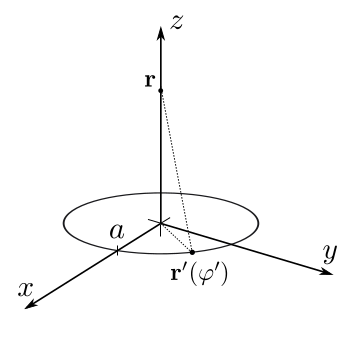
\includegraphics[width=\linewidth]{Guia1/anillo.png}
  \end{subfigure}
  \caption{Anillo cargado uniformemente}
  \label{fig:anillo}
\end{figure}

Podemos parametrizar los puntos del anillo en coordenadas polares de la siguiente manera:

$$\mathbf{r'} = a(\cos \varphi' \hat{x} + \sin \varphi' \hat{y})$$

$$\Rightarrow d\mathbf{r'} = a(-\sin \varphi' d\varphi' \hat{x} + \cos \varphi' d\varphi'\hat{y}) \Rightarrow dl' = |d\mathbf{r'}| = ad\varphi'$$

Por otro lado,

$$\mathbf{r} - \mathbf{r'} = z\hat{z} - a\cos \varphi' \hat{x} - a\sin \varphi' \hat{y} \Rightarrow |\mathbf{r} - \mathbf{r'}| = \sqrt{z^{2} + a^{2}}$$

Luego, reemplazando esto en la integral (\ref{eq:poisson_lineal}) nos da que el campo el\'ectrico en el eje del anillo es

$$\Phi_{eje}(z) = \int_{0}^{2\pi} ad\varphi' \frac{Q}{2\pi a} \frac{1}{\sqrt{z^{2} + a^{2}}} = \frac{Q}{\sqrt{z^{2} + a^{2}}}$$

Para los puntos muy lejanos al anillo ($|z| \gg a$), escribimos

$$\frac{1}{\sqrt{z^{2} + a^{2}}} = \frac{1}{|z|\sqrt{1 + \frac{a^{2}}{z^{2}}}}$$

Sea $x = \frac{a^{2}}{z^{2}}$. Si hacemos un Taylor, obtenemos que

$$\frac{1}{\sqrt{1 + x}} \approx 1 - \frac{1}{2}x$$

$$\Rightarrow \frac{1}{|z|\sqrt{1 + \frac{a^{2}}{z^{2}}}} \approx \frac{1}{|z|}\bigg(1 - \frac{1}{2}\frac{a^{2}}{z^{2}}\bigg) =  \frac{1}{|z|} - \frac{a^{2}}{2|z|^{3}}$$

$$\Rightarrow \Phi_{eje}(z) \approx \frac{Q}{|z|}$$

Entonces, para $|z| \gg a$, el potencial el\'ectrico en el eje ser\'a el de una carga puntual ubicada en el eje $z$.

Para los puntos muy cercanos al anillo ($|z| \ll a$), el desarrollo es el mismo que el anterior, solo que sacamos $a > 0$ de la ra\'iz, es decir

$$\frac{1}{\sqrt{z^{2} + a^{2}}} = \frac{1}{|a|\sqrt{1 + \frac{z^{2}}{a^{2}}}} = \frac{1}{a\sqrt{1 + \frac{z^{2}}{a^{2}}}}$$

Ahora, tomemos $x = \frac{z^{2}}{a^{2}}$. Del desarrollo de Taylor anterior, resulta

$$\frac{1}{a\sqrt{1 + \frac{z^{2}}{a^{2}}}} \approx \frac{1}{a}\bigg(1 - \frac{1}{2}\frac{z^{2}}{a^{2}}\bigg) =  \frac{1}{a} - \frac{z^{2}}{2a^{3}}$$

Como los puntos estan muy pr\'oximos al anillo, $z \rightarrow 0$, por lo tanto el segundo t\'ermino se anula y nos queda finalmente:

$$\Phi_{eje}(z) \approx \frac{Q}{a} = 2\pi\lambda$$

Lo cual tiene sentido porque en esta aproximaci\'on estar\'iamos viendo un plano cargado para $z \geq 0$.

\item En b) tenemos un disco de radio $a$ uniformemente cargado, con carga total $Q = \pi a^{2} \sigma$, y nos piden calcular el potencial sobre el eje $z$ ($\mathbf{r} = z\hat{z}$).\newline

 \begin{figure}[H]
  \centering
  \begin{subfigure}[b]{0.4\linewidth}
    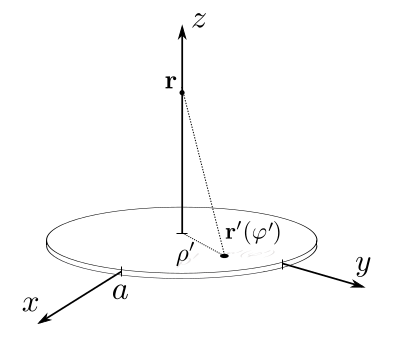
\includegraphics[width=\linewidth]{Guia1/disco.png}
  \end{subfigure}
  \caption{Disco cargado uniformemente}
  \label{fig:disco}
\end{figure}

Procedemos como en el \'item anterior, teniendo en cuenta que ahora tenemos carga superficial, por lo que usaremos (\ref{eq:poisson_sup}). Aqu\'i, una posible parametrizaci\'on de los puntos del disco en coordenadas polares es:

$$\mathbf{r'} = \rho'(\cos \varphi' \hat{x} + \sin \varphi' \hat{y})$$

$$\Rightarrow d\mathbf{r'} = (\cos \varphi' d\rho' - \rho' \sin \varphi' d\varphi')\hat{x} + (\sin \varphi' d\rho' + \rho' \cos \varphi' d\varphi')\hat{y}$$


$$\Rightarrow ds' = |d\mathbf{r'}| = \rho' d\rho' d\varphi'$$

Por otro lado,

$$\mathbf{r} - \mathbf{r'} = z\hat{z} - \rho'\cos \varphi' \hat{x} - \rho'\sin \varphi' \hat{y} \Rightarrow |\mathbf{r} - \mathbf{r'}| = \sqrt{z^{2} + \rho'^{2}}$$

Reemplazando en la integral (\ref{eq:poisson_sup}) resulta que el campo el\'ectrico en el eje del disco es

$$\Phi_{eje}(z) = \int_{0}^{2\pi} d\varphi' \int_{0}^{a} d\rho' \rho' \sigma \frac{1}{\sqrt{z^{2} + \rho'^{2}}} = 2\pi \sigma \int_{0}^{a} d\rho' \frac{\rho'}{\sqrt{z^{2} + \rho'^{2}}} = 2\pi \sigma (\sqrt{z^{2} + a^{2}} - \sqrt{z^{2}})$$

$$ \Rightarrow \Phi_{eje}(z) = 2\pi \sigma (\sqrt{z^{2} + a^{2}} - |z|)$$

Para los puntos muy lejanos ($|z| \gg a$), reescribimos la ra\'iz de este \'ultimo resultado:

$$\sqrt{z^{2} + a^{2}} = |z|\sqrt{1 + \frac{a^{2}}{z^{2}}}$$

Como $\frac{a^{2}}{z^{2}} \ll 1$ en este caso, podemos aproximarlo por $\sqrt{1 + x} \approx 1 + \frac{x}{2}$, entonces

$$|z|\sqrt{1 + \frac{a^{2}}{z^{2}}} \approx |z| + \frac{a^{2}}{2|z|}$$

Por lo cual, para puntos muy lejanos al disco, obtenemos nuevamente un potencial proporcional a $\frac{Q}{|z|}$.\newline

Ahora, para puntos cercanos al disco ($|z| \ll a$), hacemos la misma aproximaci\'on excepto que ahora el factor com\'un en la ra\'iz es $a^{2}$, por lo tanto

$$\sqrt{z^{2} + a^{2}} = |a|\sqrt{1 + \frac{z^{2}}{a^{2}}} = a\sqrt{1 + \frac{z^{2}}{a^{2}}}$$

Luego, $\frac{z^{2}}{a^{2}} \ll 1$, entonces

$$a\sqrt{1 + \frac{z^{2}}{a^{2}}} \approx a + \frac{z^{2}}{2a}$$

$$\Rightarrow \Phi_{eje}(z) = 2\pi \sigma (a + \frac{z^{2}}{2a} - |z|) = 2\pi \sigma a - 2\pi \sigma |z| - \pi \sigma \frac{z^{2}}{a}$$

Para los puntos $z \approx 0$, nos quedamos con los primeros t\'erminos de $\Phi_{eje}(z)$, por lo tanto, es proporcional al potencial de un plano cargado uniformemente, es decir:

$$\Phi_{eje}(z) \approx 2\pi \sigma a - 2\pi \sigma |z|$$

\end{itemize}

\subsection{}

En ausencia de contornos, podemos calcular el campo magn\'etico por integraci\'on directa con la ley de Biot-Savart (para densidades de corriente lineales, superficiales o volum\'etricas):

\begin{equation}
    \label{eq:biot_lineal}
    \mathbf{B(r)} = \frac{1}{c}\oint_{C} I dl' \times \frac{(\mathbf{r} - \mathbf{r'})}{|\mathbf{r} - \mathbf{r'}|^{3}}
\end{equation}

\begin{equation}
    \label{eq:biot_sup}
    \mathbf{B(r)} = \frac{1}{c}\int_{S} d^2r' \kappa(\mathbf{r'}) \times \frac{(\mathbf{r} - \mathbf{r'})}{|\mathbf{r} - \mathbf{r'}|^{3}}
\end{equation}

\begin{equation}
    \label{eq:biot_vol}
    \mathbf{B(r)} = \frac{1}{c}\int_{V} d^3r' (\mathbf{j(r')}) \times \frac{(\mathbf{r} - \mathbf{r'})}{|\mathbf{r} - \mathbf{r'}|^{3}}
\end{equation}

En este ejercicio, tenemos un solenoide de secci\'on circular de largo $L$, radio $a$ y con $n$ vueltas por unidad de longitud y corriente $I$, como muestra el esquema

\begin{figure}[H]
  \centering
  \begin{subfigure}[b]{0.6\linewidth}
    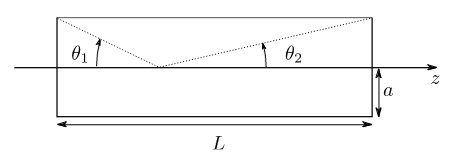
\includegraphics[width=\linewidth]{Guia1/ej4g1.png}
  \end{subfigure}
  \caption{Esquema de la configuraci\'on dada.}
  \label{fig:ej4g1}
\end{figure}

\begin{itemize}
    \item La densidad de corriente volum\'etrica ser\'a

$$\mathbf{j(r')} = \hat{\varphi}nI \theta\bigg( z' + \frac{L}{2}\bigg)\theta\bigg(\frac{L}{2} - z'\bigg)\delta(r' - a)$$

Los puntos campo y fuente nos quedan

$$\mathbf{r} = z\hat{z}$$
$$\mathbf{r'} = r'\hat{r} + z'\hat{z}$$
$$\Rightarrow \mathbf{r} - \mathbf{r'} = -r'\hat{r} + (z - z')\hat{z} \Rightarrow |\mathbf{r} - \mathbf{r'}| = \sqrt{r'^{2} + (z - z')^{2}}$$

\begin{figure}[H]
  \centering
  \begin{subfigure}[b]{0.8\linewidth}
    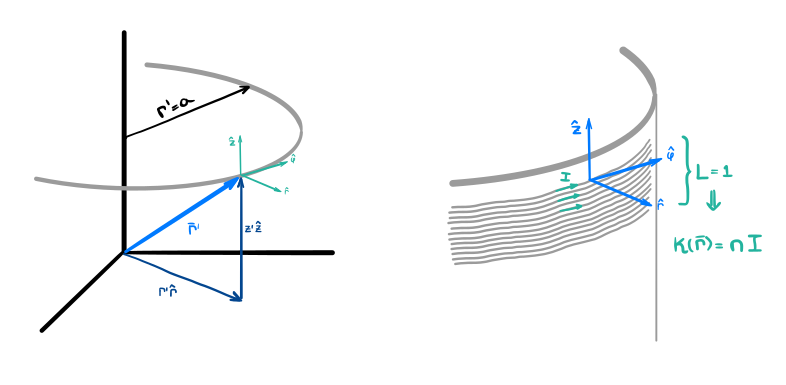
\includegraphics[width=\linewidth]{Guia1/ej4g1_2.png}
  \end{subfigure}
  \caption{Sistemas de coordenadas cil\'indricas elegido para el solenoide.}
  \label{fig:ej4g1_1}
\end{figure}

Para calcular $\mathbf{B}$ en el eje, usemos la expresi\'on (\ref{eq:biot_vol}) en coordenadas cil\'indricas con origen en el centro del cilindro:

$$\mathbf{B}(0, 0, z) = \hat{\varphi}\frac{1}{c}nI \int_{-\infty}^{+\infty}dz' \theta\bigg( z' + \frac{L}{2}\bigg)\theta\bigg(\frac{L}{2} - z'\bigg) \int_{0}^{2\pi} d\varphi'\int_{0}^{\infty} r' dr' \delta(r' - a) \times \frac{-r'\hat{r} + (z - z')\hat{z}}{(r'^{2} + (z - z')^{2})^{\frac{3}{2}}}$$

Teniendo en cuenta que las $\theta$ de Heaviside modifican los l\'imites de integraci\'on, y la $\delta$ de Dirac pone un $r' = a$ al integrar, el campo nos queda

$$\mathbf{B}(0, 0, z) = \frac{1}{c}nIa \int_{-\frac{L}{2}}^{\frac{L}{2}}dz' \int_{0}^{2\pi} d\varphi' \hat{\varphi} \times \frac{-a\hat{r} + (z - z')\hat{z}}{(a^{2} + (z - z')^{2})^{\frac{3}{2}}}$$

$$\Rightarrow \mathbf{B}(0, 0, z) = \frac{1}{c}nIa \int_{-\frac{L}{2}}^{\frac{L}{2}}dz' \int_{0}^{2\pi} d\varphi' \frac{a\hat{z} + (z - z')\hat{r}(\varphi)}{(a^{2} + (z - z')^{2})^{\frac{3}{2}}}$$

$$\Rightarrow \mathbf{B}(0, 0, z) = \frac{2\pi}{c}nIa^{2} \int_{-\frac{L}{2}}^{\frac{L}{2}}dz' \frac{\hat{z}}{(a^{2} + (z - z')^{2})^{\frac{3}{2}}} + \frac{1}{c}nIa \int_{-\frac{L}{2}}^{\frac{L}{2}}dz' \int_{0}^{2\pi} d\varphi' \frac{z - z'}{(a + (z - z')^{2})^{\frac{3}{2}}}\hat{r}(\varphi)$$

En el segundo t\'ermino, el versor $\hat{r}(\varphi)$ se puede escribir en coordenadas cartesianas como

$$\hat{r}(\varphi) = \cos \varphi \hat{x} + \sin \varphi \hat{y}$$

$$\Rightarrow \mathbf{B}_{r}(0, 0, z) = \frac{1}{c}nIa \int_{-\frac{L}{2}}^{\frac{L}{2}}dz' \int_{0}^{2\pi} d\varphi' \frac{z - z'}{(a + (z - z')^{2})^{\frac{3}{2}}}(\cos \varphi \hat{x} + \sin \varphi \hat{y}) = 0$$

ya que $\int_{0}^{2\pi} d\varphi' \sin \varphi' = \int_{0}^{2\pi} d\varphi' \cos \varphi' = 0$ \newline

Por otro lado, el primer t\'ermino lo podemos ver en tablas, y resulta

$$\mathbf{B}_{z}(0, 0, z) = \frac{2\pi}{c}nIa^{2} \int_{-\frac{L}{2}}^{\frac{L}{2}}dz' \frac{\hat{z}}{(a^{2} + (z - z')^{2})^{\frac{3}{2}}} = \frac{2\pi nIa^{2}}{c} \frac{-(z - z')}{a^{2}\sqrt{a^{2} + (z - z')^{2}}}\bigg|_{z' = -\frac{L}{2}}^{z' = \frac{L}{2}} \hat{z}$$

$$\Rightarrow \mathbf{B}_{z}(0, 0, z) = 2\pi \frac{nI}{c} \bigg[\frac{\frac{L}{2} + z}{\sqrt{(\frac{L}{2} + z)^{2} + a^{2}}} - \frac{-\frac{L}{2} + z}{\sqrt{(-\frac{L}{2} + z)^{2} + a^{2}}}\bigg]\hat{z}$$

$$ \Rightarrow \mathbf{B}(0, 0, z) = 2\pi \frac{nI}{c} (\cos \theta_{1} + \cos \theta_{2})\hat{z}$$

Cuando $L \rightarrow \infty$ (solenoide infinito), el campo nos queda

$$\lim_{L \rightarrow \infty} \mathbf{B}_{z}(0, 0, z) = 2\pi \frac{nI}{c} \lim_{L \rightarrow \infty} \bigg[\frac{\frac{L}{2} + z}{\sqrt{(\frac{L}{2} + z)^{2} + a^{2}}} - \frac{-\frac{L}{2} + z}{\sqrt{(-\frac{L}{2} + z)^{2} + a^{2}}}\bigg]\hat{z} = 2\pi \frac{nI}{c}(1 - (-1)) \hat{z} = 4\pi \frac{nI}{c}\hat{z}$$

\item Vamos a calcular el l\'imite del campo cerca del eje, para lo cual podemos expandirlo as\'i

$$B_{r}(r, z) = a_{0} + a_{r}r + a_{z}z + a_{rr}r^{2} + a_{zz}z^{2} + a_{rz}rz + ...$$

$$B_{z}(r, z) = b_{0} + b_{r}r + b_{z}z + b_{rr}r^{2} + b_{zz}z^{2} + b_{rz}rz + ...$$

Podemos usar las simetrı\'ias para encontrar algunos coeficientes. Si reflejamos respecto de $z$, tenemos simetr\'ia en la corriente, entonces

$$\mathbf{B}(r, z) = -R_{z} \mathbf{B}(r, -z) = -R_{z} (B_{z} , B_{r} , B_{\varphi})(r, -z) = (B_{z} , -B_{r} , -B_{\varphi})(r, -z)$$

En particular, $B_{r}(r, z) = -B_{r}(r, -z) \Rightarrow a_{0} = a_{r} = a_{rr} = a_{zz} = 0$. Adem\'as, ya sabemos que $B_{z}(r, z) = -B_{z}(r, -z) \Rightarrow b_{z} = b_{rz} = 0$ y como calculamos en el \'item anterior $B_{r}(0, 0, z) = 0$, entonces $a_{z} = 0$. \newline

Por el momento, tenemos

$$B_{r}(r, z) = a_{rz}rz + ...$$

$$B_{z}(r, z) = b_{0} + b_{r}r + b_{z}z + b_{rr}r^{2} + b_{zz}z^{2} + ...$$

Para ver los t\'erminos restantes, utilicemos la divergencia del campo magn\'etico, es decir:

$$\nabla \cdot \mathbf{B} = \frac{1}{r}\frac{\partial}{\partial r}(rB_{r}) + \frac{\partial B_{z}}{\partial z} = 0$$

$$\Rightarrow \frac{1}{r}\frac{\partial}{\partial r}(ra_{rz}rz) + \frac{\partial}{\partial z}(b_{0} + b_{r}r + b_{z}z + b_{rr}r^{2} + b_{zz}z^{2}) = 0$$

$$\Rightarrow 2a_{rz}z + 2b_{zz}z = 0 \Rightarrow a_{rz} = -b_{zz}$$

Usando el rotor de $\mathbf{B}$,

$$(\nabla \times \mathbf{B})_{\varphi} = 0 = \frac{\partial}{\partial z}B_{r} - \frac{\partial}{\partial r}B_{z}$$

$$\Rightarrow \frac{\partial}{\partial z}(a_{rz}rz) - \frac{\partial}{\partial r}(b_{0} + b_{r}r + b_{z}z + b_{rr}r^{2} + b_{zz}z^{2})$$

$$\Rightarrow 0 = a_{rz}r - (b_{r} + 2b_{rr}r)$$

Luego, $a_{rz} = 2b_{rr}$, $b_{r} = 0$. En resumen, obtenemos lo siguiente de cada componente del campo:

$$B_{r}(r, z) = -b_{zz}rz + ...$$

$$B_{z}(r, z) = b_{0} -\frac{1}{2}b_{zz}r^{2} + b_{zz}z^{2} + ...$$

El t\'ermino que nos interesa es justamente $b_{zz}$, f\'acil de calcular

$$b_{zz} = \frac{1}{2}\frac{\partial^{2}}{\partial z^{2}}B_{z}|_{r = z = 0} = -\frac{\pi n I}{c}\frac{3a^{2}L}{(\frac{L^{2}}{4} + a^{2})^{\frac{5}{2}}}$$

Por lo tanto, el m\'odulo del campo cerca del origen es

$$B_{r}(r, z) \approx \frac{\pi n I r z}{c}\frac{3a^{2}L}{(\frac{L^{2}}{4} + a^{2})^{\frac{5}{2}}}$$

Si $a \ll L$, obtenemos el resultado pedido en el ejercicio

$$B_{r}(r, z) \approx \frac{96\pi n I}{c}\bigg( \frac{a^{2}rz}{L^{4}}\bigg)$$

\end{itemize}

\subsection{}

\begin{itemize}
    \item Tenemos que encontrar la densidad de carga de un \'atomo de hidr\'ogeno en el estado fundamental, con el siguiente potencial generado por el n\'ucleo puntual y la nube electr\'onica

    $$\Phi(r) = \frac{q}{r}\bigg(1 + \frac{r}{a} \bigg)e^{-\frac{2r}{a}}$$

    donde $a$ es el radio de Bohr y $q$ la carga del prot\'on. Podr\'iamos utilizar la ecuaci\'on de Poisson $\nabla^{2} \Phi = -4\pi \rho$,  y calcular el laplaciano en esf\'ericas, pero hay que tener cuidado porque tenemos un potencial que es singular en el origen. \newline

    En efecto, el laplaciano en esf\'ericas para un potencial que depende solo de la coordenada radial nos queda

    $$\nabla^{2} \Phi(r) = \frac{1}{r^{2}}\frac{\partial}{\partial r}\bigg(r^{2}\frac{\partial \Phi}{\partial r} \bigg)$$

    La aplicaci\'on directa de esta expresi\'on a un potencial de la forma $\frac{q}{r}$ dar\'ia 0, cuando su resultado correcto ser\'ia $-4\pi q \delta^{3}(\mathbf{r})$ (por ser el potencial de una carga puntual en el origen). Para resolver esto, escribamos el potencial como la suma de una parte singular y otra regular, es decir

    $$\Phi(r) = q(g_{S} + g_{R})$$

    $$\Rightarrow \nabla^{2} \Phi(r) = q(\nabla^{2} g_{S}(r) + \nabla^{2} g_{R}(r)$$

    Para la parte singular, basta con tomar $g_{S}(r) = \frac{1}{r}$, por lo tanto su laplaciano ser\'a $\nabla^{2} g_{S}(r) = -4\pi q \delta^{3}(\mathbf{r})$.\newline

    Por otro lado, la parte regular se puede escribir como $g_{R}(r) = \Phi(r) - g_{S}(r) = \frac{1}{r}[(1 + \frac{r}{a})e^{-\frac{2r}{a}} - 1]$, luego $\nabla^{2} g_{R}(r) = \frac{4}{a^{3}}e^{-\frac{2r}{a}}$.\newline

    En definitiva, la densidad de carga resulta

    $$\rho = -\frac{1}{4\pi}\nabla^{2} \Phi(r) = q\bigg[\delta^{3}(\mathbf{r}) - \frac{1}{\pi a^{3}}e^{-\frac{2r}{a}}\bigg]$$

    \item El primer t\'ermino (la delta en el origen) se identifica con la densidad de carga $\rho_{q}$ del prot\'on, el segundo t\'ermino puede interpretarse como la densidad $\rho_{e}$ de la nube electr\'onica.

    \item Para ver que la distribuci\'on corresponde a un \'atomo neutro, notemos que si integramos la densidad de carga de la nube electr\'onica, obtenemos $-q$:

    $$\int d^{3}r \rho_{e}(r) = -4\pi \int_{0}^{\infty}dr r^{2} \frac{q}{\pi a^{3}}e^{-\frac{2r}{a}} = -4q \int_{0}^{\infty} dx x^{2} e^{-2x} = -q$$

    \item El campo el\'ectrico para $r > 0$ sale de la ecuaci\'on

    $$\mathbf{E} = -\nabla \Phi(r) = -q\nabla(g_{S} + g_{R}) = -q\nabla g_{S} - q\nabla g_{R}$$

    En coordenadas esf\'ericas, la coordenada radial del gradiente tiene la siguiente expresi\'on

    $$\nabla \Phi(r) = \frac{\partial \Phi}{\partial r}\hat{r}$$

    Sabemos que
    
    $$g_{S}(r) = \frac{1}{r} \Rightarrow \frac{\partial g_{S}}{\partial r} = -\frac{1}{r^{2}}$$

    $$g_{R}(r) = \Phi(r) - g_{S}(r) = \frac{1}{r}[(1 + \frac{r}{a})e^{-\frac{2r}{a}} - 1] \Rightarrow \frac{\partial g_{R}}{\partial r} = \frac{1}{r^{2}} - \frac{e^{-\frac{2r}{a}}(a^{2} + 2ar + 2r^{2})}{(ra)^{2}}$$

    Juntando todos estos resultados en $\mathbf{E}$ nos queda que

    $$\mathbf{E} = \bigg[\frac{q}{r^{2}} - \frac{q}{r^{2}} + q\frac{e^{-\frac{2r}{a}}(a^{2} + 2ar + 2r^{2})}{(ra)^{2}}\bigg]\hat{r} = q\frac{e^{-\frac{2r}{a}}(a^{2} + 2ar + 2r^{2})}{(ra)^{2}}\hat{r}$$
    
\end{itemize}

\subsection{}

En este problema, tenemos un cilindro infinito de radio $a$ con densidad uniforme de carga, excepto a lo largo de una cavidad cil\'indrica de radio $b$, paralela al eje del cilindro. El eje de la cavidad está\'a una distancia $d$ del eje del cilindro, tal que $d + b < a$. \newline

\begin{figure}[H]
  \centering
  \begin{subfigure}[b]{0.8\linewidth}
    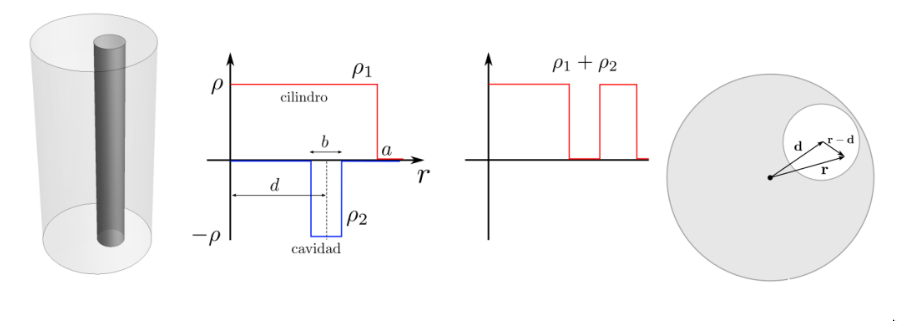
\includegraphics[width=\linewidth]{Guia1/g1e6.png}
  \end{subfigure}
  \caption{Disposici\'on del cilindro y la cavidad en su interior.}
  \label{fig:g1e6}
\end{figure}


Vamos a calcular este problema con el principio de superposici\'on, tomando a la densidad de carga de la cavidad $\rho_{2} = -\rho$.\newline

\begin{itemize}
    \item Tomando una superficie de Gauss, calculamos el campo de un cilindro macizo cualquiera

$$\oint_{C_{r}} \mathbf{E}_{CM} \cdot d\mathbf{S} = 4\pi Q_{enc}$$

Si $r \leq a$, entonces

$$E_{CM}(\mathbf{r})2\pi|\mathbf{r}|L = 4\pi(\rho \pi|\mathbf{r}|^{2}L) \Rightarrow E_{CM}(\mathbf{r}) = 2\pi \rho |\mathbf{r}|$$

Si $r > a$,

$$E_{CM}(\mathbf{r})2\pi|\mathbf{r}|L = 4\pi(\rho \pi a^{2}L) \Rightarrow E_{CM}(\mathbf{r}) = 2\pi \rho \frac{a^{2}}{|\mathbf{r}|}$$

En resumen,

 \[\mathbf{E}_{CM}(\mathbf{r})=
        \begin{cases}
            2\pi \rho |\mathbf{r}|\hat{r} =  2\pi \rho \mathbf{r}& r \leq a\\
             2\pi \rho \frac{a^{2}}{|\mathbf{r}|}\hat{r} = 2\pi \rho \frac{a^{2}}{|\mathbf{r}|^{2}}\mathbf{r}  & r > a
        \end{cases}
    \]

Ahora que tenemos este resultado general, el campo $\mathbf{E}_{1}$ ser\'a el del cilindro de radio $a$ y $\mathbf{E}_{2}$ el de la cavidad hueca de radio $b$, m\'as precisamente

$$\mathbf{E}_{1} = \mathbf{E}_{CM}(\mathbf{r})$$

$$\mathbf{E}_{2} = \mathbf{E}_{CM}(\mathbf{r} - \mathbf{d})$$

$$\Rightarrow \mathbf{E} = \mathbf{E}_{1} + \mathbf{E}_{2}$$

Dentro de la cavidad (que a su vez est\'a dentro del cilindro), el campo es

$$\mathbf{E(r)} = 2\pi \rho \mathbf{r} + 2\pi \rho(\mathbf{r} - \mathbf{d}) = cte$$

\item En el \'item b) nos dan un cilindro donde circula una corriente total $I$. El campo magn\'etico del cilindro completo es

$$B2\pi r = \oint_{c_{r}} \mathbf{B} \cdot d\mathbf{l} = \frac{4\pi}{c}I_{enc} = \frac{4\pi}{c}I \frac{\pi r^{2}}{\pi a^{2}}$$

$$\mathbf{B}_{1}(\mathbf{r}) = \frac{2Ir}{ca^{2}}\hat{\varphi} = \frac{2I}{ca^{2}} \hat{z} \times \mathbf{r}$$

Por otro lado, el campo del cilindro desplazado (con corriente opuesta) ser\'a

$$\mathbf{B}_{2}(\mathbf{r}) = \frac{2Ir}{ca^{2}}\hat{\varphi} = -\frac{2I}{ca^{2}} \hat{z} \times (\mathbf{r - d})$$

Por el principio de superposici\'on, el campo magn\'etico total resulta

$$\mathbf{B(r)} = \mathbf{B}_{1}(\mathbf{r}) + \mathbf{B}_{2}(\mathbf{r}) = \frac{2I}{ca^{2}} \hat{z} \times \mathbf{d}$$

\end{itemize}

\subsection{}

\begin{itemize}
    \item Nuevamente, por superposici\'on, nos piden hallar el campo y el potencial electrost\'atico producido por dos hilos paralelos, infinitos, uniformemente cargados con $\lambda = \lambda_{1} = -\lambda_{2}$.

    \begin{figure}[H]
  \centering
  \begin{subfigure}[b]{0.5\linewidth}
    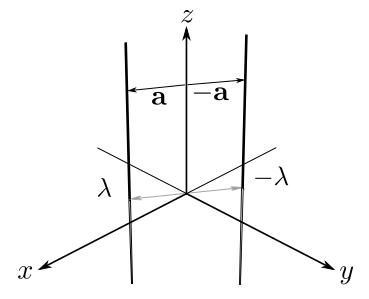
\includegraphics[width=\linewidth]{Guia1/g1e7.png}
  \end{subfigure}
  \caption{Dos hilos paralelos e infinitos, cada uno separado una distancia $a$ del origen.}
  \label{fig:g1e7}
\end{figure}

Sabiendo que el campo y potencial el\'ectrico de un hilo infinito en el eje $z$ son

$$\mathbf{E(r)} = \frac{2\lambda}{\rho}\hat{\rho}$$

$$\Phi(r) = -2\lambda \ln \bigg( \frac{\rho}{\rho_{0}}\bigg)$$

Como los hilos est\'an desplazados del eje por un vector $\mathbf{a}$ en el plano $xy$, la distancia del punto $r$ a cada hilo ser\'a $|\mathbf{\rho} - \mathbf{a}|$, y el versor que da la direcci\'on del campo el\'ectrico es $\frac{(\mathbf{\rho} - \mathbf{a})}{|\mathbf{\rho} - \mathbf{a}|}$.\newline

Por lo tanto, para el hilo desplazado en $\mathbf{a}$, obtenemos

$$\mathbf{E(r)} = \frac{2\lambda}{|\mathbf{\rho} - \mathbf{a}|}\frac{(\mathbf{\rho} - \mathbf{a})}{|\mathbf{\rho} - \mathbf{a}|} = 2\lambda \frac{(\mathbf{\rho} - \mathbf{a})}{|\mathbf{\rho} - \mathbf{a}|^{2}}$$

$$\Phi(r) = -2\lambda \ln \bigg( \frac{|\mathbf{\rho} - \mathbf{a}|}{|\mathbf{\rho_{0}} - \mathbf{a}|}\bigg)$$

Con esto, podemos sumar las soluciones para los dos hilos (uno en $a$ con densidad $\lambda$, y el otro en $-a$ con densidad $-\lambda$:

$$\mathbf{E(r)} = 2\lambda \bigg(\frac{(\mathbf{\rho} - \mathbf{a})}{|\mathbf{\rho} - \mathbf{a}|^{2}} - \frac{(\mathbf{\rho} + \mathbf{a})}{|\mathbf{\rho} + \mathbf{a}|^{2}}\bigg)$$

$$\Phi(r) = -2\lambda \bigg[\ln \bigg( \frac{|\mathbf{\rho} - \mathbf{a}|}{|\mathbf{\rho_{0}} - \mathbf{a}|}\bigg) - \ln \bigg( \frac{|\mathbf{\rho} + \mathbf{a}|}{|\mathbf{\rho_{0}} + \mathbf{a}|}\bigg)\bigg] = 2\lambda \ln \bigg( \frac{|\mathbf{\rho} + \mathbf{a}|}{|\mathbf{\rho} - \mathbf{a}|}\bigg)$$.\newline

\item Para hallar los equipotenciales, tomamos la \'ultima ecuaci\'on del punto anterior y laa igualamos a una constante

$$\Phi(r) = 2\lambda \ln \bigg( \frac{|\mathbf{\rho} + \mathbf{a}|}{|\mathbf{\rho} - \mathbf{a}|}\bigg) = V$$

Las curvas determinadas por esta ecuaci\'on son c\'irculos, lo que implica que las superficies equipotenciales son cilindros circulares (haciendo los despejes correspondientes. Para m\'as detalle, consultar la demostraci\'on en el apunte de Zanella). Debajo se muestra un esquema de dichas equipotenciales

  \begin{figure}[H]
  \centering
  \begin{subfigure}[b]{0.5\linewidth}
    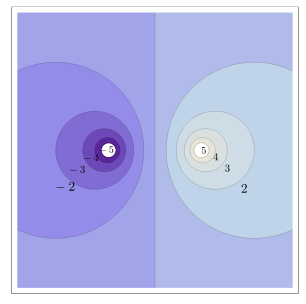
\includegraphics[width=\linewidth]{Guia1/g1e7_equip.png}
  \end{subfigure}
  \caption{Superficies equipotenciales de dos hilos paralelos e infinitos (con densidades $\lambda$ y $-\lambda$), equidistantes.}
  \label{fig:g1e7_equip}
\end{figure}

\item En c) proponen resolver el problema de dos cilindros del mismo radio, a potenciales opuestos, separados por una distancia mayor que la suma de sus radios. Este problema puede encararse pensando en una situaci\'on equivalente de dos hilos con $\lambda$ y -$\lambda$, de manera que las equipotenciales de los cables a $V_{1}$ y $V_{2}$ coincidieran con las superficies de los cilindros.

\begin{figure}[H]
  \centering
  \begin{subfigure}[b]{0.6\linewidth}
    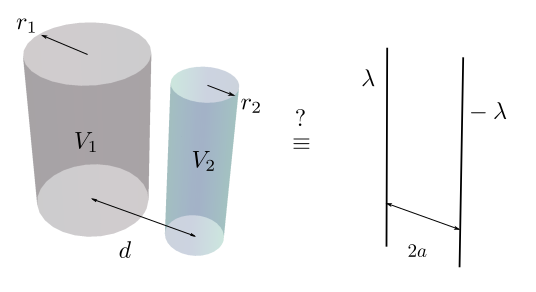
\includegraphics[width=\linewidth]{Guia1/g1e7_cil.png}
  \end{subfigure}
  \caption{Esquema del problema de los dos cilindros, equivalente al de los dos hilos con condiciones de contorno adecuadas.}
  \label{fig:g1e7_cil}
\end{figure}

Nuevamente, la explicaci\'on detallada est\'a en el apunte de Zanella.

\end{itemize}

\subsection{}

\begin{itemize}
    \item En este punto tenemos una esfera met\'alica a tierra (de radio $b$) rodeada por una c\'ascara esf\'erica (de radio $a$) con una densidad de carga uniforme $\sigma$.

\begin{figure}[H]
  \centering
  \begin{subfigure}[b]{0.3\linewidth}
    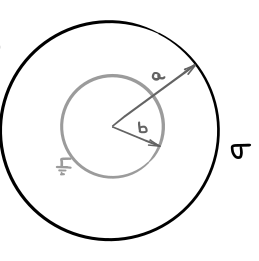
\includegraphics[width=\linewidth]{Guia1/ej8g1.png}
  \end{subfigure}
  \caption{Esfera met\'alica a tierra, rodeada por una c\'ascara esf\'erica.}
  \label{fig:ej8g1}
\end{figure}

Ya sabemos que el potencial de una c\'ascara esf\'erica de radio $a$ con densidad uniforme $\sigma$ se escribe de la siguiente manera

\[\Phi_{c\'ascara}(r)=
        \begin{cases}
            \frac{Q}{a} & r < a\\
             \frac{Q}{r}  & r > a
        \end{cases}
    \]

con $Q = 4\pi a^{2} \sigma$. Esto no puede ser la soluci\'on del problema completo porque no satisface la condici\'on de contorno $\Phi(r = b) = 0$, debido a que el cascar\'on cargado junto a esta condici\'on inducen una densidad de carga $\sigma_{ind}$ en la superficie de la esfera a tierra de radio $b$.\newline

Usemos el principio de superposici\'on, separando el problema original como muestra el esquema

\begin{figure}[H]
  \centering
  \begin{subfigure}[b]{0.95\linewidth}
    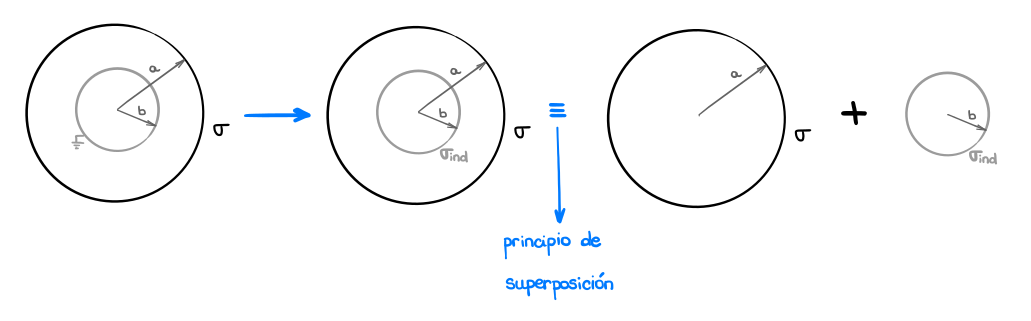
\includegraphics[width=\linewidth]{Guia1/ej8g1_sup1.png}
  \end{subfigure}
  \caption{Configuraci\'on equivalente a la original.}
  \label{fig:ej8g1_sup1}
\end{figure}

Entonces, el potencial total ser\'a

$$\Phi(r) = \Phi_{\sigma}(r) + \Phi_{\sigma_{ind}}(r) = 
        \begin{cases}
            \frac{Q}{a} & r < a\\
             \frac{Q}{r}  & r > a
        \end{cases}
    +  \begin{cases}
            \frac{Q_{ind}}{b} & r < b\\
             \frac{Q_{ind}}{r}  & r > b
        \end{cases} = 
        \begin{cases}
            \frac{Q}{a} + \frac{Q_{ind}}{b} & r < b\\
             \frac{Q}{a} + \frac{Q_{ind}}{r}  & b < r < a \\
             \frac{Q}{r} + \frac{Q_{ind}}{r}  & r > a
        \end{cases}$$

donde $Q = 4\pi a^{2} \sigma$ y $Q_{ind} = 4\pi b^{2} \sigma_{ind}$.\newline

Para hallar $\sigma_{ind}$, pedimos que se anule el potencial en $r = b$, es decir

$$\Phi(r = b) = 0 \Rightarrow \frac{4\pi a^{2} \sigma}{a} + \frac{4\pi b^{2} \sigma_{ind}}{b} = 0$$

$$\Rightarrow \sigma_{ind} = -\sigma \frac{a}{b}$$

Reemplazando este resultado en el potencial total, nos queda finalmente

\[\Phi(r) = \begin{cases}
            0 & r < b\\
             \frac{4\pi \sigma a^{2}}{a} - \frac{4\pi \sigma ab}{r}  & b < r < a \\
             4\pi \sigma\frac{a^{2} - ab}{r} & r > a
        \end{cases}
        \]

\item Queremos usar el principio de superposici\'on en los siguientes tres casos

\begin{figure}[H]
  \centering
  \begin{subfigure}[b]{0.8\linewidth}
    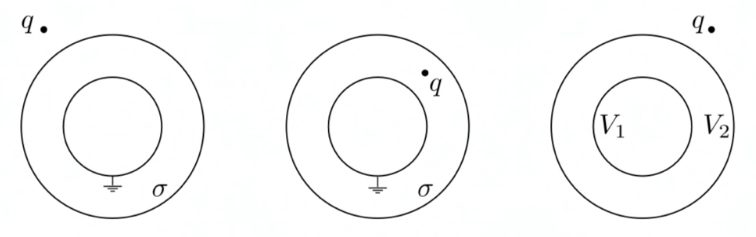
\includegraphics[width=\linewidth]{Guia1/ej8g1_sup2.png}
  \end{subfigure}
  \caption{Configuraciones del problema.}
  \label{fig:ej8g1_sup2}
\end{figure}

Suponiendo conocidos los resultados del \'item anterior m\'as el potencial producido por una carga frente a una esfera a tierra, las posibles soluciones son

\begin{figure}[H]
  \centering
  \begin{subfigure}[b]{0.95\linewidth}
    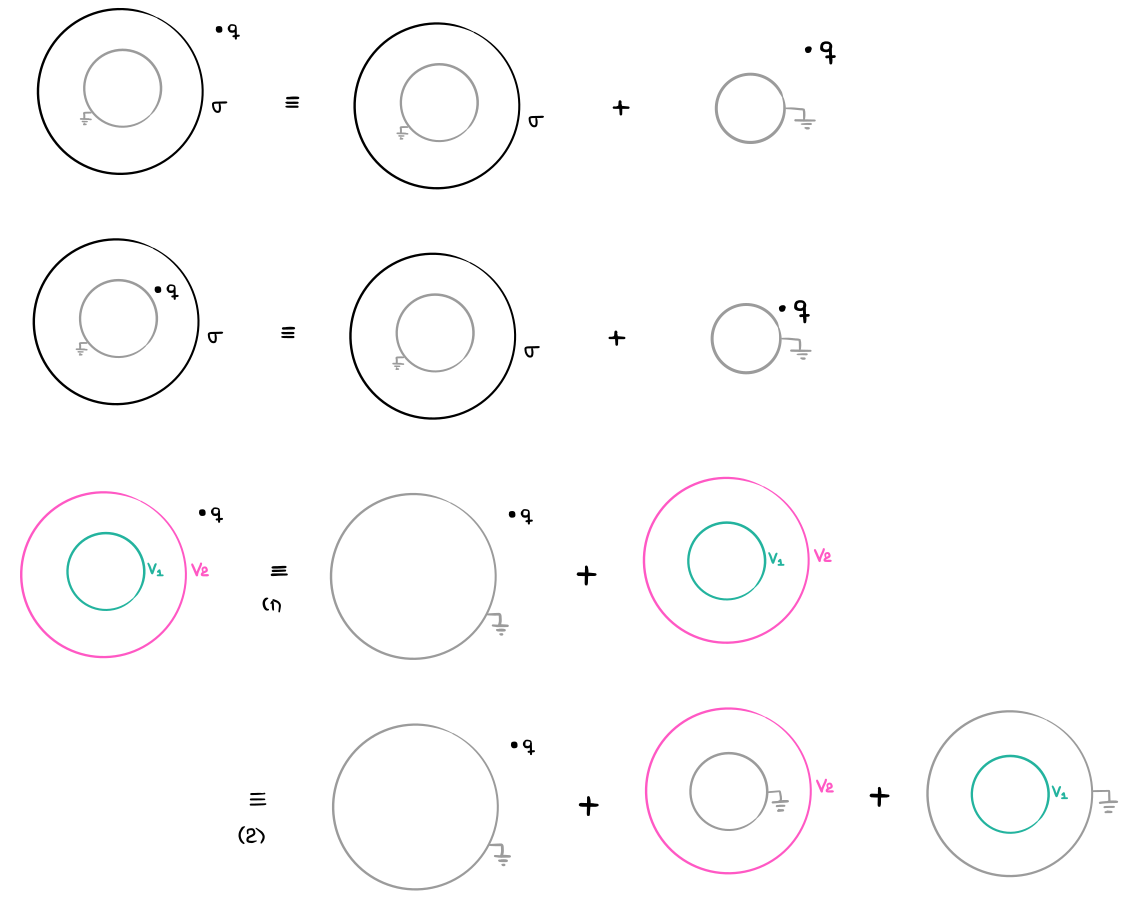
\includegraphics[width=\linewidth]{Guia1/ej8g1_sup3.png}
  \end{subfigure}
  \caption{Posibles soluciones para cada una de las configuraciones del problema. Notemos que (1) y (2) son dos versiones equivalentes del mismo problema que, ahora si, respetan las condiciones de contorno al superponer los potenciales.}
  \label{fig:ej8g1_sup3}
\end{figure}

\end{itemize}



\newpage
\section{M\'etodo de im\'agenes, funci\'on de Green y separaci\'on de variables}

\subsection{}
En este problema, tenemos una esfera conductora de radio $a$ conectada a un potencial $V$, rodeada por otra c\'ascara esf\'erica de radio $b$ con densidad superficial de carga $\sigma$

\begin{figure}[H]
  \centering
  \begin{subfigure}[b]{0.7\linewidth}
    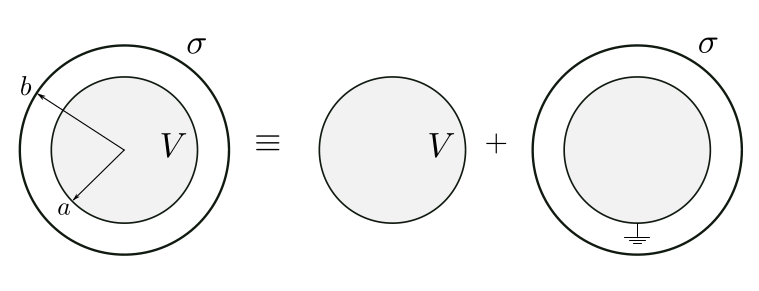
\includegraphics[width=\linewidth]{Guia2/g2_e1_im.png}
  \end{subfigure}
  \caption{Diagrama de la configuraci\'on dada.}
  \label{fig:g2_e1_im}
\end{figure}

\begin{itemize}
    \item En el punto a) queremos hallar $\Phi$ en todo el espacio usando el m\'etodo de im\'agenes con la superposici\'on propuesta en la figura (\ref{fig:g2_e1_im}). Esto nos permite escribir el potencial como la siguiente suma:

    $$\Phi(\mathbf{r}) = \Phi_{CC}(\mathbf{r}) + \Phi_{\sigma}(\mathbf{r})$$

    donde $\Phi_{CC}(\mathbf{r})$ es el potencial de la esfera a $V$ y $\Phi_{\sigma}(\mathbf{r})$ el del cascar\'on con densidad $\sigma$ y la esfera a tierra.

    El potencial $\Phi_{CC}$ decae como $\frac{1}{r}$ fuera de la esfera, y es igual a $V$ dentro de ella, luego por continuidad debe ser $\frac{Va}{r}$. Si utilizamos la notaci\'on  
    
    $$r_{>~}^{(a)} = max[r, a]$$

    Dicho potencial nos quedar\'a finalmente

    $$\Phi_{CC}(\mathbf{r}) = \frac{Va}{r_{>~}^{(a)}}$$

    donde $Va$ es la carga inducida sobre la esfera a potencial $V$.\\
    
    Para el potencial de la c\'ascara y la esfera a tierra, $\Phi_{\sigma}$, podemos tomar a cada elemento infinitesimal de la c\'ascara como una carga puntual con una carga imagen asociada (dentro de la c\'ascara). Particularmente, como todos los puntos son equivalentes, cada imagen se encuentra a la misma distancia del origen, es decir

    $$r' = \frac{a^{2}}{b}$$

    Por \'ultimo, para $r \geq a$, el potencial de la c\'ascara frente a la esfera es el potencial de dos c\'ascaras: una de radio $b$ y carga $Q$ y su imagen de radio $r'$ y carga $Q' = -\frac{a}{b}Q$:

    \[\Phi_{\sigma}(\mathbf{r})=
        \begin{cases}
            \frac{Q'}{r_{>~}^{(r')}} + \frac{Q}{r_{>~}^{(b)}} = Q\bigg(-\frac{a}{br} + \frac{1}{r_{>~}^{(b)}}\bigg) & r \geq a\\
            0  & r \leq a
        \end{cases}
    \]

    donde $r_{>~}^{(r')} = r$ en la regi\'on $r \geq a$. Luego, el potencial total del problema ser\'a

    \[\Phi(\mathbf{r}) = \Phi_{CC}(\mathbf{r}) + \Phi_{\sigma}(\mathbf{r})
        \begin{cases}
            \frac{Va}{r} Q\bigg(-\frac{a}{br} + \frac{1}{r_{>~}^{(b)}}\bigg) & r \geq a\\
            V & r \leq a
        \end{cases}
    \]

    \item La carga total inducida sobre la esfera ser\'a

    $$Q_{TOT} = Va + Q'$$
\end{itemize}

\subsection{}
Veamos el problema anterior pero utilizando la funci\'on de Green. La mayoría de las veces vamos a utilizar las condiciones de contorno de Dirichlet, entonces podemos escribir el potencial electrost\'atico de la siguiente manera

\begin{equation}
    \label{eq:green_dirichlet}
    \Phi(\mathbf{r}) = \int_{V}d^{3}\mathbf{r}'\rho(\mathbf{r}')G(\mathbf{r}, \mathbf{r}') - \frac{1}{4\pi}\oint_{S}d^{2}r'\frac{\partial G(\mathbf{r}, \mathbf{r}')}{\partial n'}\Phi(\mathbf{r}')
\end{equation}

donde el valor del potencial en $S$ es dato.\newline

Como en el problema, si las cargas en volumen est\'an distribuidas sobre una superficie $\Sigma$, el primer t\'ermino de (\ref{eq:green_dirichlet}) es una integral de superficie

$$\int_{V}d^{3}\mathbf{r}'\rho(\mathbf{r}')G(\mathbf{r}, \mathbf{r}') = \int_{\Sigma}d^{2}r'\sigma(\mathbf{r}')G(\mathbf{r}, \mathbf{r}')$$

En nuestro caso, las integrales que est\'an sobre las superficies de radio $a$ (contorno) y $b$ (cargas), quedan

$$\int_{\Sigma}d^{2}r' \rightarrow \int_{r' = a, b}d^{2}r'$$

Adem\'as, como el volumen del problema es en la regi\'on $r > a$, la normal exterior es $\mathbf{n}' = -\hat{r}'$, luego $\frac{\partial}{\partial n'} = -\frac{\partial}{\partial r'}$. Con toda esta informaci\'on, la ecuaci\'on (\ref{eq:green_dirichlet}) nos queda

\begin{equation}
    \label{eq:green1}
    \Phi(\mathbf{r}) = \int_{r' = b}d^{2}r'G(\mathbf{r}, \mathbf{r}')\sigma + \frac{V}{4\pi}\int_{r' = a}d^{2}r'\frac{\partial G(\mathbf{r}, \mathbf{r}')}{\partial r'}
\end{equation}

Luego, la funci\'on de Green correspondiente es

\begin{equation}
    \label{eq:green2}
    G(\mathbf{r}, \mathbf{r}') = \frac{1}{|\mathbf{r} - \mathbf{r}'|} - \frac{a}{r'}\frac{1}{|\mathbf{r} - \frac{a^{2}}{r'^{2}}\mathbf{r}'|}
\end{equation}

En este punto, hay varios m\'etodos para resolver la ecuaci\'on (\ref{eq:green1}), vamos a utilizar la expansi\'on en arm\'onicos esf\'ericos de la funci\'on de Green. La primer integral de dicha ecuaci\'on puede escribirse en funci\'on del \'angulo s\'olido de la siguiente manera

$$ \Phi_{V}(\mathbf{r}) = \int_{r' = b}d^{2}r'G(\mathbf{r}, \mathbf{r}')\sigma = \int_{r' = b}b^{2}d\Omega G(\mathbf{r}, \mathbf{r}')\sigma$$

donde la integral angular es sobre el vector $\mathbf{r}'$

$$\int d\Omega \rightarrow \int_{0}^{2\pi} d\phi' \int_{-1}^{1}\sin \theta' d\theta'$$

La funci\'on de Green expresada en arm\'onicos esf\'ericos es

\begin{equation}
    \label{eq:green3}
    G(\mathbf{r}, \mathbf{r}') = \sum_{lm} \frac{4\pi}{2l + 1}Y_{lm}(\theta, \phi)Y_{lm}^{*}(\theta', \phi')\bigg[ \frac{r^{l}_{<~}}{r^{l+1}_{>~}} - \frac{a^{2l + 1}}{(rr')^{l+1}}\bigg]
\end{equation}

$$\Rightarrow \Phi_{V}(\mathbf{r}) = \sum_{lm} \frac{4\pi \sigma}{2l + 1}\bigg[ \frac{r^{l}_{<~}}{r^{l+1}_{>~}} - \frac{a^{2l + 1}}{(rr')^{l+1}}\bigg]_{r' = b}\bigg[Y_{lm}(\theta, \phi)\int b^{2}d\Omega Y_{lm}^{*}(\theta', \phi')\bigg]$$

Un buen truco es escribir la integral de $Y_{lm}^{*}(\theta', \phi')$ como el producto escalar con $1 = \sqrt{4\pi}Y_{00}(\theta', \phi')$, entonces $\int b^{2}d\Omega Y_{lm}^{*}(\theta', \phi') = \sqrt{4\pi}\int b^{2}d\Omega Y_{lm}^{*}(\theta', \phi')Y_{00}(\theta', \phi') = \sqrt{4\pi}\delta_{l, 0}\delta_{m, 0}$.\\

Luego en $\Phi_{V}(\mathbf{r})$ quedan solo los t\'erminos con $m = l = 0$, entonces

$$\Phi_{V}(\mathbf{r}) = 4\pi b ^{2}\sigma\bigg[ \frac{1}{r_{>~}} - \frac{a}{br}\bigg] = Q\bigg[ \frac{1}{r_{>~}} - \frac{a}{br}\bigg]$$\\

La contribuci\'on del potencial en la superficie es

$$ \Phi_{S}(\mathbf{r}) = \frac{V}{4\pi}\int_{r' = a}d^{2}r'\frac{\partial G(\mathbf{r}, \mathbf{r}')}{\partial r'}$$\\

Ac\'a tenemos que $r_{<~} = r'$ y $r_{>~} = r$, por lo tanto

$$\Phi_{S}(\mathbf{r}) = \frac{V}{4\pi} \sum_{lm} \frac{4\pi}{2l + 1}(2l + 1) \frac{a^{l - 1}}{r^{l+1}}\bigg[ Y_{lm}(\theta, \phi)\int a^{2} d\Omega Y_{lm}^{*}(\theta', \phi')\bigg] = \frac{Va}{r}$$

\subsection{}
En la siguiente im\'agen vemos un esquema del problema

\begin{figure}[H]
  \centering
  \begin{subfigure}[b]{0.3\linewidth}
    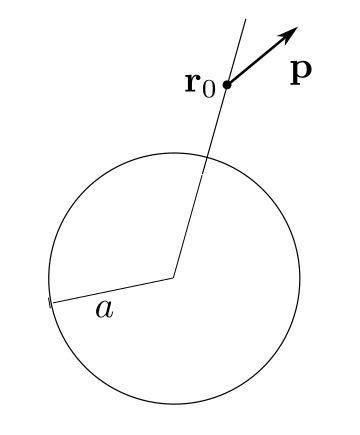
\includegraphics[width=\linewidth]{Guia2/g2_dipolo.png}
  \end{subfigure}
  \caption{Diagrama de la configuraci\'on.}
  \label{fig:g2_dipolo}
\end{figure}


donde $\mathbf{p}$ es un dipolo ubicado en el punto $\mathbf{r}_{0}$ junto a una esfera de radio $a$. Tenemos que calcular el potencial en todo el punto del espacio

\begin{itemize}
    \item M\'etodo de la funci\'on de Green

    \item M\'etodo de im\'agenes
\end{itemize}



%----------------------------------------------------------------------------------------


%----------------------------------------------------------------------------------------
%	REFERENCE LIST
%----------------------------------------------------------------------------------------
%\newpage
%\begin{thebibliography}{99} % Bibliography - this is intentionally simple in this template
 
%\end{thebibliography}


%----------------------------------------------------------------------------------------

\end{document}